\documentclass[12pt]{beamer}
\newenvironment{ConCodigo}[1]
  {\begin{frame}[fragile,environment=ConCodigo]{#1}}
  {\end{frame}}
\graphicspath{{Imagenes/}{../Imagenes/}}
\usepackage[utf8]{inputenc}
\usepackage[spanish]{babel}
\usepackage{hyperref}
\usepackage{etex}
%\reserveinserts{28}
\usepackage{amsmath}
\usepackage{amsthm}
\usepackage{mathtools}
\usepackage{multicol}
\usepackage{multirow}
\usepackage{tabulary}
\usepackage{booktabs}
\usepackage{nccmath}
\usepackage{physics}
\usepackage{biblatex}
\usepackage[outdir=./]{epstopdf}
%\epstopdfsetup{outdir=./}
\usepackage{graphicx}
%\usepackage{enumitem,xcolor}
\usepackage{siunitx}
%\sisetup{scientific-notation=true}
%\usepackage{fontspec}
\usepackage{lmodern}
\usepackage{float}
\usepackage[format=hang, font=footnotesize, labelformat=parens]{caption}
\usepackage[autostyle,spanish=mexican]{csquotes}
\usepackage{standalone}
\usepackage{blkarray}
\usepackage{algorithm}
\usepackage{algorithmic}
\usepackage{tikz}
\usepackage[siunitx, RPvoltages]{circuitikz}
\usetikzlibrary{arrows,patterns,shapes}
\usetikzlibrary{decorations.markings}
\usetikzlibrary{arrows}
\usepackage{color}
\usepackage{xcolor}
%\usepackage{beton}
%\usepackage{euler}
%\usepackage[T1]{fontenc}
\usepackage[sfdefault]{roboto}  %% Option 'sfdefault' only if the base font of the document is to be sans serif
\usepackage[T1]{fontenc}
\renewcommand*\familydefault{\sfdefault}
\DeclareGraphicsExtensions{.pdf,.png,.jpg}
\usepackage{hyperref}
\renewcommand {\arraystretch}{1.5}
\newcommand{\python}{\texttt{python}}
\usefonttheme[onlymath]{serif}
\setbeamertemplate{navigation symbols}{}
\usetikzlibrary{patterns}
\usetikzlibrary{decorations.markings}
\tikzstyle{every picture}+=[remember picture,baseline]
%\tikzstyle{every node}+=[inner sep=0pt,anchor=base,
%minimum width=2.2cm,align=center,text depth=.15ex,outer sep=1.5pt]
%\tikzstyle{every path}+=[thick, rounded corners]
\setbeamertemplate{caption}[numbered]
\newcommand{\ptm}{\fontfamily{ptm}\selectfont}
%Se usa la plantilla Warsaw modificada con spruce
\mode<presentation>
{
  \usetheme{Warsaw}
  \setbeamertemplate{headline}{}
  \useoutertheme{default}
  \usecolortheme{albatross}
  \setbeamercovered{invisible}
}
% \AtBeginSection[]
% {
% \begin{frame}<beamer>{Contenido}
% \normalfont\mdseries
% \tableofcontents[currentsection]
% \end{frame}
% }

\usefonttheme[onlymath]{serif}
\include{pre_codigo}
\begin{document}
\title{Tema 0 - Programación Básica con \python \\ Clase 2}
\subtitle{Curso de Física Computacional}
\author[]{M. en C. Gustavo Contreras Mayén}
\date{ }
\maketitle
\fontsize{14}{14}\selectfont
\spanishdecimal{.}
\begin{frame}
\frametitle{Contenido}
\tableofcontents[pausesections]
\end{frame}
\section{Estructuras de control}
\begin{frame}
\frametitle{Estructuras de control}
En cualquier lenguaje de programación se incluye una serie de estructuras de control para ampliar las posibilidades de ejecución de un programa.
\\
\bigskip
Manejaremos las más comunes que son relativamente sencillas de usar, cuidado siempre de manejar la sintaxis respectiva.
\end{frame}
\subsection{Condicionales}
\begin{frame}
\frametitle{Condicionales}
Una sentencia condicional permite evaluar si se cumple cierta condición, es decir, si su valor es \texttt{True}, se ejecuta una instrucción, en caso de que el valor de la condición no se cumpla, valor \texttt{False}, no se ejecuta la instrucción contenida y se sigue a la siguiente línea de código.
\end{frame}
\begin{frame}
\frametitle{El condicional \texttt{if}}
El bloque condicional más simple utiliza la instrucción \texttt{if}, a continuación lleva una expresión que debe de evaluarse, como se mencionó antes, el valor de la expresión debe de ser \texttt{True} para que se ejecute(n) la(s) instrucción(es) contenidas en el bloque, hay dos puntos (:) que identifican el bloque y las instrucciones contenidas deben de estar identadas, en caso contrario, \python\ nos devolverá un mensaje de error provocado por la identación equivocada.
\end{frame}
\begin{frame}[fragile]
\frametitle{Ejemplo de \texttt{if}}
\begin{lstlisting}
a = 10
if a > 0:
    print 'la variable a es positiva'
    a = a + 1

print a
\end{lstlisting}
\fontsize{12}{12}\selectfont
En el ejemplo asignamos a la variable \texttt{a} el valor de 10, en el bloque condicional se evalúa la expresión \texttt{a > 10}, y en este caso, el valor que se obtiene es \textcolor{red}{\texttt{True}}, por tanto, se ejecutan las instrucciones que están contenidas dentro del bloque, que son: 1) mostrar en pantalla la línea \texttt{la variable a es positiva}, 2) se incrementa una unidad el valor de \texttt{a}. Aquí ya concluyen las instrucciones dentro del condicional, la siguiente instrucción \texttt{print} está fuera del bloque, y nos muestra el valor de la variable \texttt{a}, que en el ejemplo ahora es 11.
\end{frame}
\begin{frame}[fragile]
\frametitle{Cuando la expresión evaluada es falsa}
\begin{lstlisting}
a = 0
if a > 0:
    print 'la variable a es positiva'
    a = a + 1

print a
\end{lstlisting}
Ahora vemos que el valor de la variable \texttt{a} es cero, y al evaluarse la expresión \texttt{a > 10}, el resultado es \textcolor{blue}{False}, por tanto NO se ejecuta instrucción alguna que está dentro del bloque, y continua el código hacia la siguiente línea, en el ejemplo, con la instrucción \texttt{print}.
\end{frame}
\begin{frame}
\frametitle{Alternativa 1 para el bloque condicional}
En ocasiones necesitaremos hacer algo cuando la expresión que se evalúa en el \texttt{if} sea falsa, el programa realice alguna instrucción, es decir, que haya una respuesta en particular para el caso en que obtengamos un valor \texttt{False} en la evaluación de la expresión.
\\
\medskip
Para ello, podemos ocupar la instrucción \texttt{else:} que se escribe en el mismo nivel de identación que la instrucción \texttt{if} y lleva también dos puntos (:); las instrucciones que están contenidas dento de \texttt{else:} se ejecutarán siempre y cuando la expresión que se evalúa, sea falsa, \python\ no pide otra expresión para evaluar.
\end{frame}
\begin{frame}[fragile]
\frametitle{Condicional \texttt{if .. else}}
\begin{lstlisting}
a = -2
if a > 0:
    print 'la variable a es positiva'
    a = a + 1
else:
	print 'la variable a es negativa'
print a
\end{lstlisting}
\fontsize{12}{12}\selectfont
En el ejemplo vemos que el valor de \texttt{a} es $-2$, la expresión que se evalúa en el \texttt{if} es \textcolor{blue}{\texttt{False}}, por tanto, no se ejecutan las instrucciones del \texttt{if}, sino que se va a ejecutar la instrucción contenida en el \texttt{else:}
\\
\medskip
Si la expresión inicial que se evaluá es \textcolor{red}{\texttt{True}}, se ejecutan las instrucciones contenidas en el bloque \texttt{if}, ya no se ejecuta instrucción alguna del bloque \texttt{else:} y continua el programa.
\end{frame}
\begin{frame}
\frametitle{Alternativa 2 para el bloque condicional}
El uso de un bloque \texttt{if .. else} nos da oportunidad manejar el código en caso de obtener un valor \texttt{False} en la evaluación de la expresión, como ya mencionamos, no se requiere evaluar otra expresión, pero podemos usar una variante del condicional y evaluar una nueva expresión (que sería diferente de la primera) y con ello, nuestro algoritmo gana bastante potencial para responder a nuestras necesidades, y eso lo haremos con el bloque \texttt{if .. elif .. else}
\end{frame}
\begin{frame}[fragile]
\frametitle{El bloque \texttt{if..elif..else}}
\begin{lstlisting}
a = 0
if a > 0:
    print 'la variable a es positiva'
    a = a + 1
elif a == 0:
    print 'la variable a es cero'
else:
    print 'la variable a es negativa'

print a
\end{lstlisting}
\fontsize{12}{12}\selectfont
La primera expresión \texttt{a>0} es \textcolor{blue}{\texttt{False}}, por tanto, continua el código hasta la sentencia \texttt{elif:}, aquí se evalúa la nueva expresión \texttt{a == 0}, que resulta ser \textcolor{red}{\texttt{True}} y por tanto se ejecuta la instrucción contenida en el bloque \texttt{elif:}, saliendo luego del bloque y continua el código, es decir, ya no se revisa el \texttt{else:}
\end{frame}
\begin{frame}[fragile]
\frametitle{Ejemplo de condicional}
\begin{lstlisting}
a = input('Introduce el valor de a')
if a > 0:
    print "a es positivo"
    a = a + 1
elif a == 0:
    print "a es 0"
else:
    print "a es negativo"

print a:
\end{lstlisting}
\end{frame}
\begin{frame}[fragile]
\frametitle{Uso de los condicionales}
Para imprimir formas plurales
\begin{lstlisting}
print "Hay % d % s en el banco " % \
(N, (" peso " if N == 1 else " pesos "))
\end{lstlisting}
\pause
Para funciones por tramos
\begin{lstlisting}
y = (x if x < 10.0 else (x**2)/10.0)
\end{lstlisting}
\pause
Para evaluar funciones condicionalmente
\begin{lstlisting}
def Perim ( radius ): return 2* pi* radius
def Area ( radius ): return pi* radius **2
v = ( Perim if q == 'perim ' else Area )(1.0)
\end{lstlisting}
\end{frame}
\subsection{Bucles o Loops}
\begin{frame}
\frametitle{Bucles o Loops}
Un bucle es una sentencia que evalúa inicialmente una condición, en caso de que se cumple (valor \texttt{True}) se ejecuta(n) un conjunto de instrucciones, posteriormente, se revisa el valor de la condición, mientras sea verdadero, las instrucciones se ejecutan nuevamente.
\end{frame}
\begin{frame}
\frametitle{Tipos de bucles}
Hay que considerar dos posibles casos en el manejo de los bucles:
\begin{enumerate}
\item Cuando conocemos el número de ciclos que van a realizarse.
\item Cuando no sabemos cuántas veces se requiere que se repita el ciclo.
\end{enumerate}
En ambos casos se necesita modificar alguna variable y evaluar nuevamente una condición, de tal manera que se cumpla con cierto criterio y concluya el bucle, en caso contrario, tendremos lo que se denomina un \emph{bucle infinito}, es decir, el conjunto de instrucciones se va a repetir indefinidamente, por lo que hay que ''cortar'' el programa en ejecución.
\end{frame}
\subsubsection{El bucle \texttt{while}}
\begin{frame}[fragile]
\frametitle{El ciclo \texttt{while}}
El ciclo \texttt{while} tiene la siguiente sintaxis:
\\
\medskip
\begin{verbatim}
while condicion:
    instruccion1
    instruccion2
    ....
\end{verbatim}
Las instrucciones contenidas en el bloque se van a ejecutar mientras el valor de la condición sea verdadero, para salir del ciclo, el valor de la condición debe devolver \textcolor{blue}{\texttt{False}}, por lo que es necesario que dentro de este bloque, se realice alguna modificación a la(s) variable(s) contenida(s) en la condición.
\end{frame}
\begin{frame}[fragile]
\frametitle{Ejemplo del ciclo \texttt{while:}}
\begin{lstlisting}
nMax = 5
n = 1
a = [] 
while n < nMax:
    a.append(1.0/n) 
    n = n + 1
print a
\end{lstlisting}
\end{frame}
\begin{frame}[fragile]
\frametitle{Otro ejemplo del ciclo \texttt{while:}}
\begin{minipage}{5.5cm}
\begin{lstlisting}
from random import random
x = 0.2
while x < 0.6:
    x = random()
    print x
print "Acabo el bucle"
\end{lstlisting}
\end{minipage}
\hspace{1cm}
\pause
\begin{minipage}{4cm}
\texttt{
0.452132471948
0.492677330538
0.539594612795
0.0865775779807
0.0861402799157
0.96555312462
Acabó el bucle
}
\end{minipage}
\end{frame}
\subsubsection{El bucle \texttt{for}}
\begin{frame}[fragile]
\frametitle{El bucle \texttt{for}}
La sintaxis del bucle/ciclo \texttt{for} es la siguiente:
\\
\medskip
\begin{verbatim}
for variable in lista:
    instruccion1
    instruccion2
    ...
\end{verbatim}
El conjunto de instrucciones contenidas dentro del bucle se va a ejecutar mientras no se acabe de recorrer la lista; el valor de la variable, será el elemento de la lista que está siendo tratado en ese momento:
\end{frame}
\begin{frame}[fragile]
\frametitle{Ejemplo del ciclo \texttt{for}}
\begin{minipage}{5cm}
\begin{lstlisting}
cubos =[]
for i in range(7):
    ic = i**3
    cubos.append(ic)
    print i, cubos
\end{lstlisting}
\end{minipage}
\pause
\\
\medskip
\texttt{
0 [0] \\
1 [0, 1] \\
2 [0, 1, 8] \\
3 [0, 1, 8, 27] \\
4 [0, 1, 8, 27, 64] \\
5 [0, 1, 8, 27, 64, 125] \\
6 [0, 1, 8, 27, 64, 125, 216]
}
\end{frame}
\begin{frame}[fragile]
\frametitle{Algunas cosas más sobre el ciclo \texttt{for}}
La instrucción \texttt{for} no sólo itera sobre enteros: \texttt{for} itera sobre todos los elementos de una \emph{secuencia}, asignando el valor del elemento a la variable, en el ejemplo anterior, la función \texttt{range} es sólo una función conveniente que genera una lista de enteros.
\begin{verbatim}
for i in [ 3, 1, 4, 1, 5, 9, 2, 6, 5, 3 ]:
print "Un digito de pi es", i
\end{verbatim}
\begin{verbatim}
for i in [ 1, 2, 3, 4 ] + [ 3, 2, 1 ]:
print i
\end{verbatim}
\begin{verbatim}
for i in " estas son palabras al azar ".split ():
print i
\end{verbatim}
\end{frame}
\begin{frame}[fragile]
\frametitle{Ejemplos del ciclo \texttt{for}}
\begin{lstlisting}
for i in range(10):
    print i
\end{lstlisting}
Al usar la función \texttt{range},  podemos extender el uso del ciclo \texttt{for}
\begin{lstlisting}
for i in range(1,10):
    print i

for j in range(10,1,-1):
    print j

lista = ['adios', 'mundo', 'cruel']
for palabra in lista:
    print palabra
\end{lstlisting}
\end{frame}
\begin{frame}[fragile]
\frametitle{Ciclo \texttt{for} más elaborado}
El siguiente código usa los elementos de lista y busca la coincidencia exacta del nombre que proporciona el usuario en la línea de comandos, en caso de que no lo encuentre, le avisa al usuario que ese nombre no está en la lista inicial.
\begin{lstlisting}
lista = ['Hugo', 'Paco', 'Luis', 'McPato']
nombre = raw_input('Teclea un nombre: ')

for i in range(len(lista)):
    if lista[i] == nombre:
    	print nombre, ' es el numero ', i + 1, ' en la lista'
    break
else:
    print nombre, ' no esta en la lista'
\end{lstlisting}
\end{frame}
\begin{frame}
\frametitle{El uso de \texttt{else} en el bloque \texttt{for}}
En el ejemplo anterior, vemos que hay una sentencia \texttt{else:} al mismo nivel de alineación del ciclo \texttt{for}, efectivamente, esta sentencia \texttt{else:} no pertenece al condicional \texttt{if}, sino al bloque \texttt{for}.
\\
\medskip
La sentencia \texttt{else:} la podemos utilizar tanto para los bucles \texttt{for} y \texttt{while}.
\end{frame}
\begin{frame}
\frametitle{Instrucciones \texttt{break} y \texttt{continue}}
Hay dos instrucciones que permiten ''salirse'' de un bucle sin necesidad de esperar a que en un ciclo \texttt{while}, la expresión que se evalúa, cambie a un valor \textcolor{blue}{False}, y para un ciclo \texttt{for}, esperar a que se recorran todos los elementos de la lista.
\\
\medskip
La instrucción es \texttt{break}, veamos en el siguiente ejemplo, cómo se usa.
\end{frame}
\begin{frame}[fragile]
\frametitle{Uso de la instrucción \texttt{break}}
\begin{lstlisting}
for n in range(2, 10):
    for x in range(2, n):
        if n % x == 0:
            print n, ' es igual a ', x, '*', n/x
            break
    else:
        print n, ' es numero primo'
\end{lstlisting}
\end{frame}
\begin{frame}
Tenemos dos ciclos \texttt{for} anidados (hay que tener siempre cuidado con la identación) y en el segundo ciclo, tenemos un condicional \texttt{if} contenido, se evalúa con la función módulo, para expresar que un número es producto de otro, y tenemos la instrucción \texttt{break}, que no se espera a que se complete el recorrido de los elementos de la lista con índice \texttt{x}, que va desde 2 hasta n, y continua con un incremento en el contador n del primer ciclo \texttt{for}, en caso de que no haya un residuo igual a cero, entonces el número es primo, aquí nos apoyamos en la sentencia \texttt{else} del ciclo \texttt{for}.
\end{frame}
\begin{frame}[fragile]
\frametitle{Uso de la instrucción \texttt{continue}}
La instrucción \texttt{continue}, lo que hace, es dar paso a la siguiente iteración del ciclo, veamos el ejemplo:
\begin{lstlisting}
for num in range(2,10):
    if num % 2 == 0:
        print 'Encontre un numero par ', num
        continue
    print 'Encontre un numero ', num
\end{lstlisting}
\end{frame}
\section{Control de errores}
\begin{frame}[fragile]
\frametitle{Control de errores}
Cuando comenzamos a programar, nos podemos encontrar con mensajes de error al momento de ejecutar el programa, siendo las causas más comunes:
\begin{itemize}[<+->]
\item errores de dedo, escribiendo incorrectamente una instrucción, sentencia, variable o constante.
\item errores al momento de introducir los datos, por ejemplo, si el valor que se debe de ingresar es $123.45$, y si nosotros tecleamos $1234.5$, el resultado ya se considera un error.
\item errores que se muestran en tiempo de ejecución, es decir, todo está bien escrito y los datos están bien introducidos, pero hay un error debido a la lógica del programa o del método utilizado, ejemplo: división entre cero.
\end{itemize}
\end{frame}
\begin{frame}[fragile]
\frametitle{Manejo de errores}
\verb|c = 12.0/0.0| \\
\pause
\begin{exampleblock}{}
\verb|Traceback (most recent call last):| \\
\verb|File ''<pyshell#0>'', line 1, in ?| \\
\verb|c = 12.0/0.0| \\
\verb|ZeroDivisionError: float division|
\end{exampleblock}
\pause
\begin{exampleblock}{}
\verb|try:| \\
\verb|     c = 12.0/0.0| \\
\verb|except ZeroDivisionError:| \\
\verb|     print 'Division entre cero'|
\end{exampleblock}
\end{frame}
\section{Uso de Intefases de Desarrollo -IDE-}
\begin{frame}
\frametitle{Por qué usar una interfaz de desarrollo?}
Para el desarrollo de problemas científicos con \python, hemos visto y recurrido a la sintaxis y estrucutras de control propias del lenguaje, así como ejecutar un programa (o script) desde la terminal.
\\
\medskip
Cada vez, nuestros códigos aumentarán de tamaño y el riesgo también se incrementa, si omitimos alguna instrucción o dejamos un bloque sin identar, no cerramos un paréntesis, etc. Además, la interacción con varias terminales en linux, hace más complicado el orden y control.
\end{frame}
\begin{frame}
Tenemos disponibles bajo licencia GNU, varios IDEs para programar con \python. La ventaja es que precisamente integran mucho el trabajo que tenemos que hacer a mano, resalta con colores las instrucciones, nos ofrece ventanas para visualizar los resultados, sin necesidad de tener abiertas varias terminales.
\end{frame}
\begin{frame}
\frametitle{Usando \texttt{gEdit}}
\texttt{gedit} es un editor de textos compatible con UTF-8 para GNU/Linux, Mac OS X y Microsoft Windows. Diseñado como un editor de textos de propósito general, \texttt{gedit} enfatiza la simplicidad y  facilidad de uso. Incluye herramientas para la edición de código fuente y textos estructurados, como lenguajes de marcado.
\\
\medskip
Es el editor predeterminado de GNOME.
\\
\medskip
Distribuido bajo las condiciones de la licencia GPL, \texttt{gedit} es software libre.\\
\medskip
\texttt{https://wiki.gnome.org/Apps/Gedit}
\end{frame}
\begin{frame}[fragile]
\begin{figure}
	\centering
	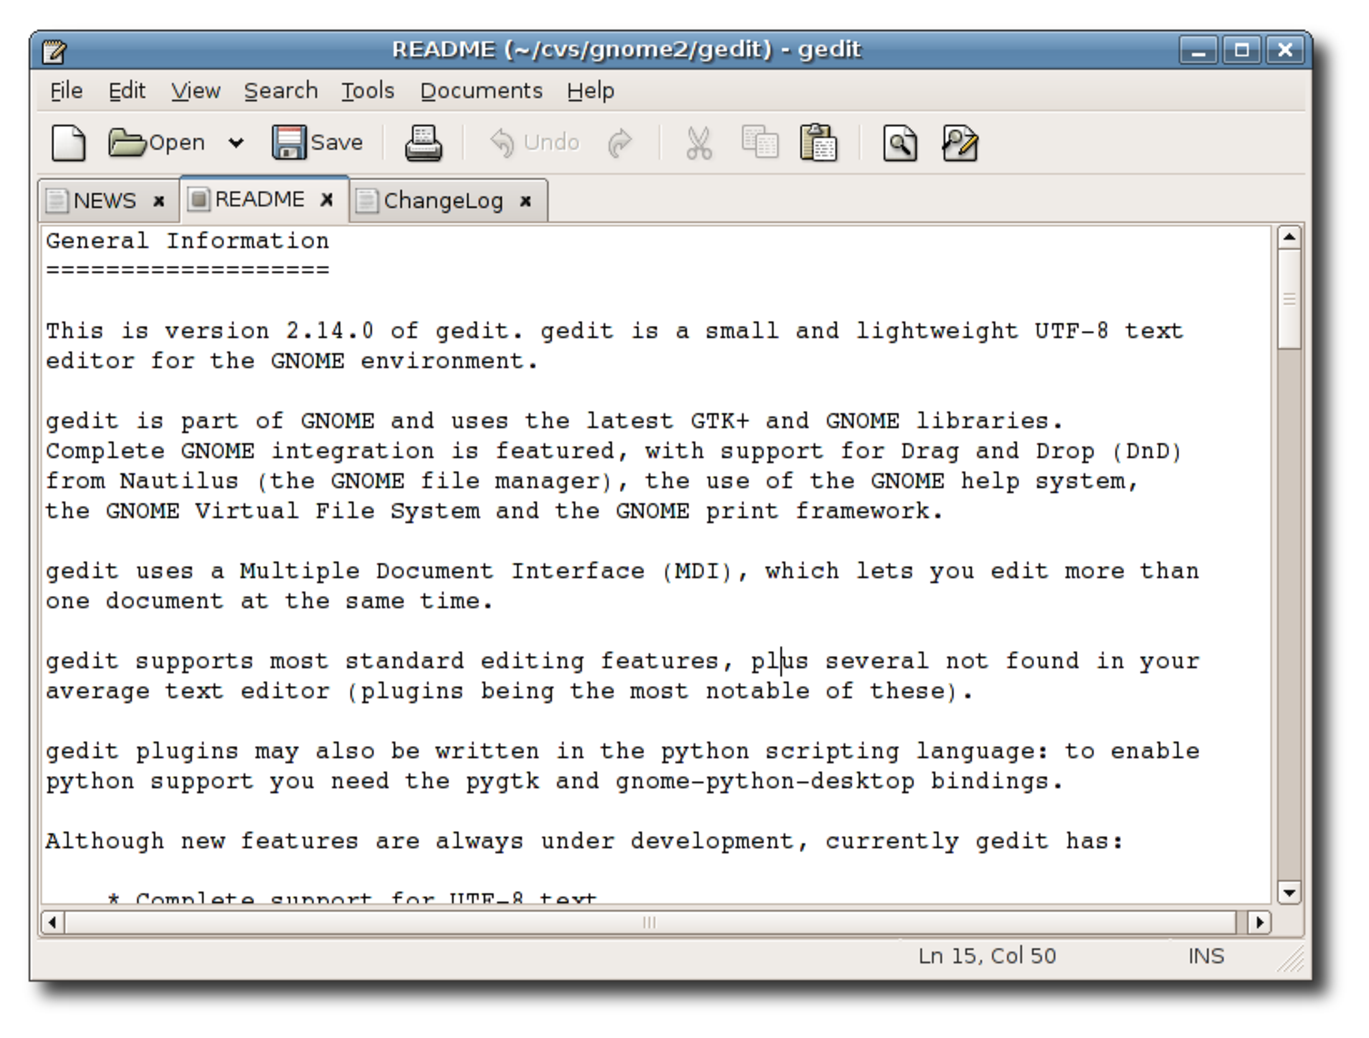
\includegraphics[scale=0.5]{gedit1.eps}<1> 
	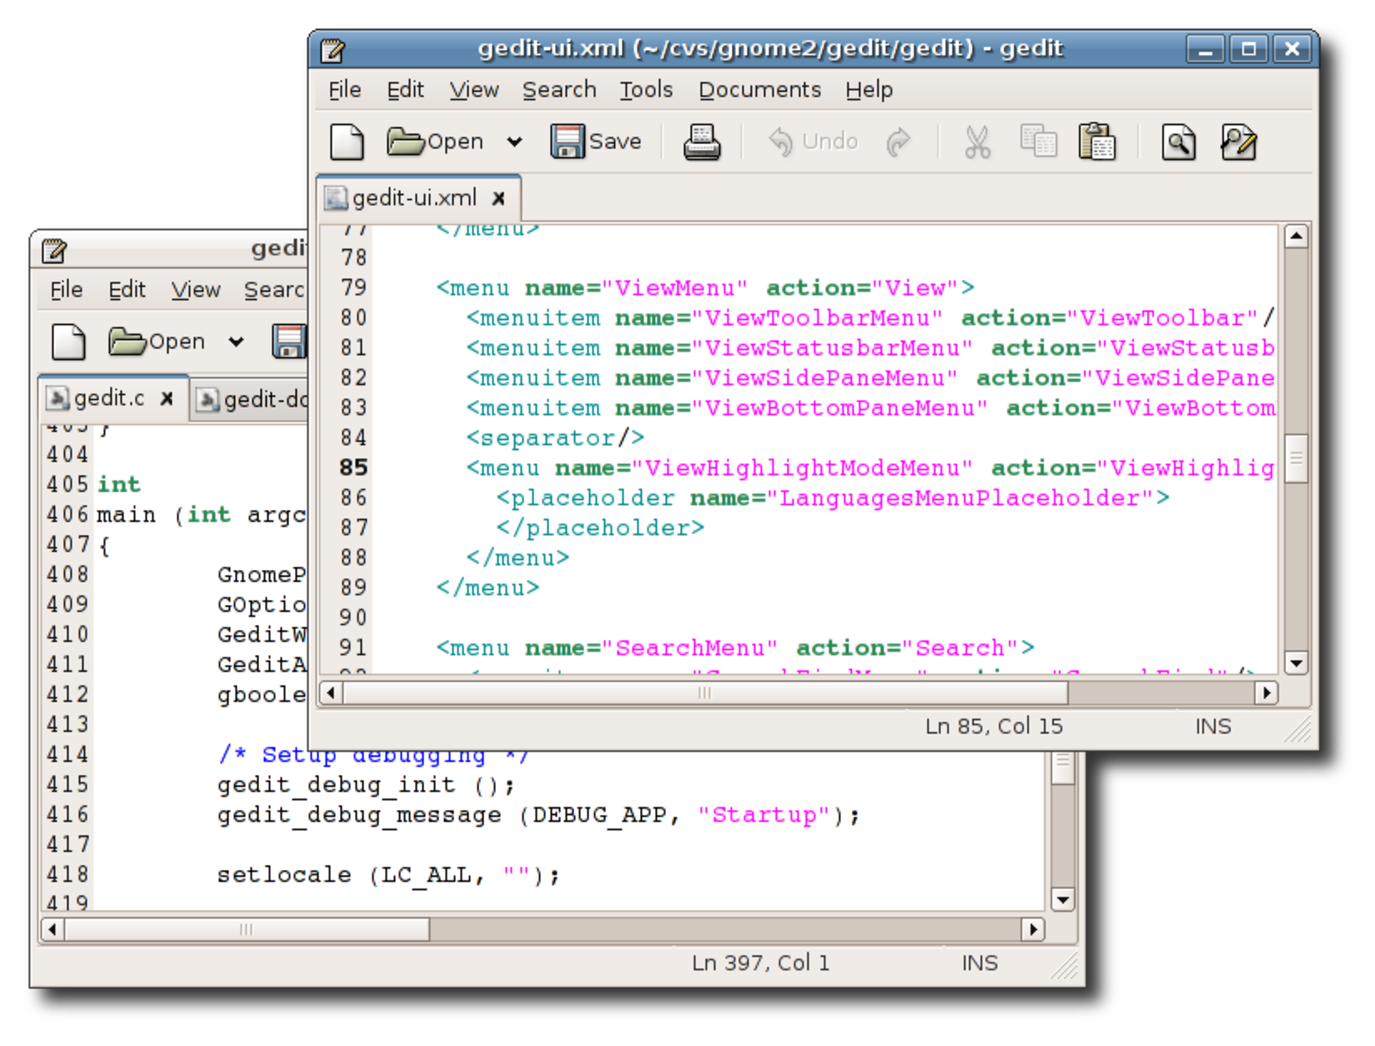
\includegraphics[scale=0.5]{gedit2.eps}<2>
	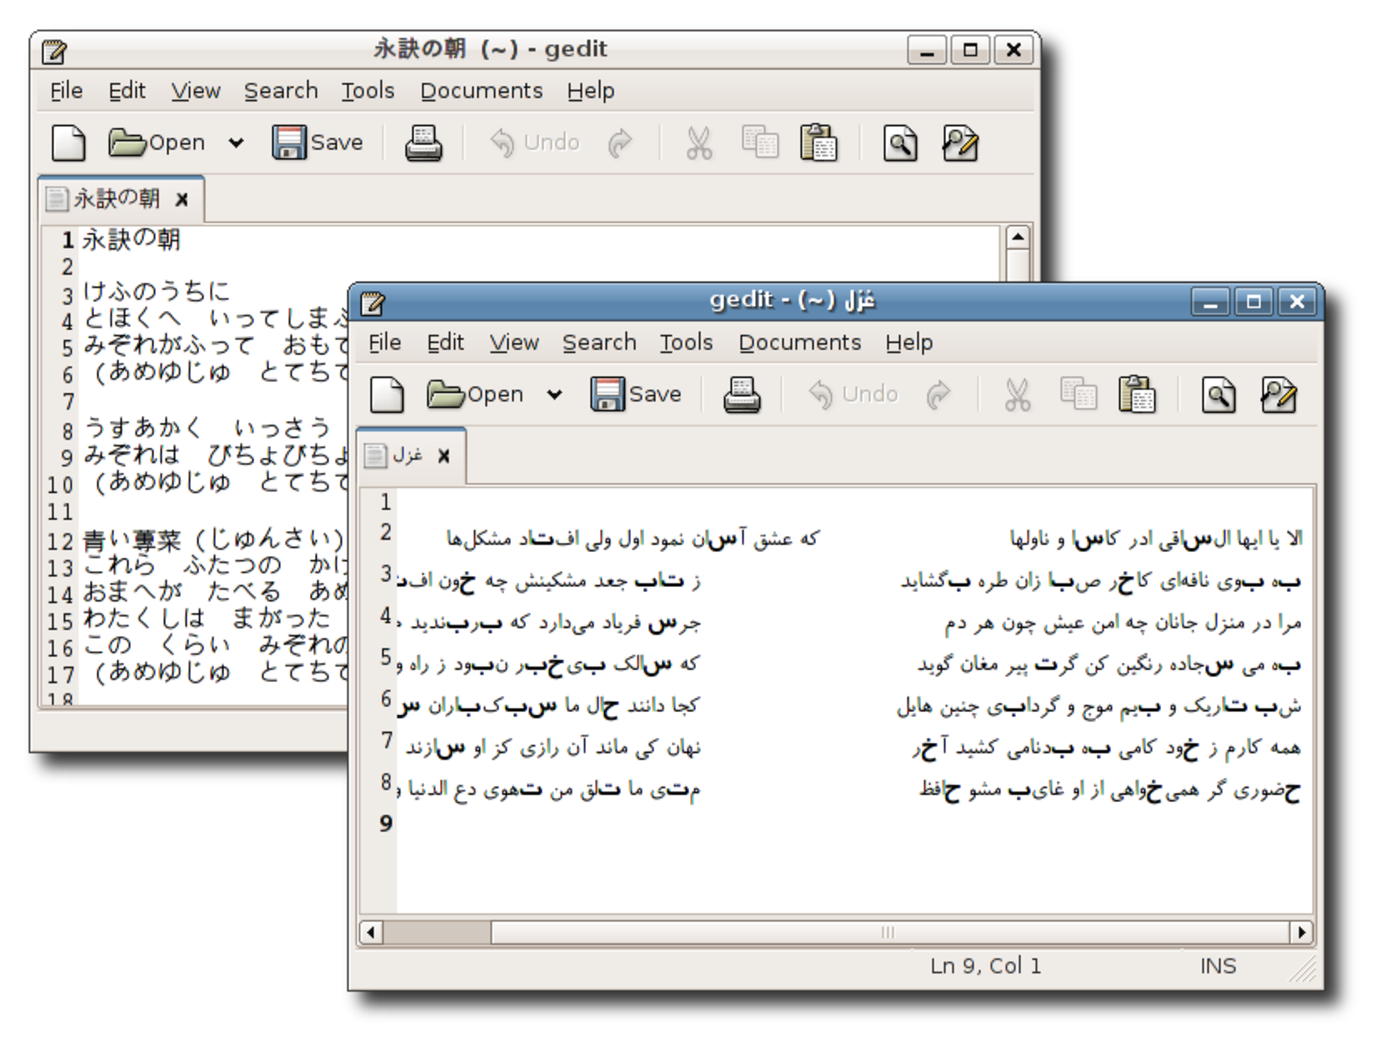
\includegraphics[scale=0.5]{gedit3.eps}<3>
	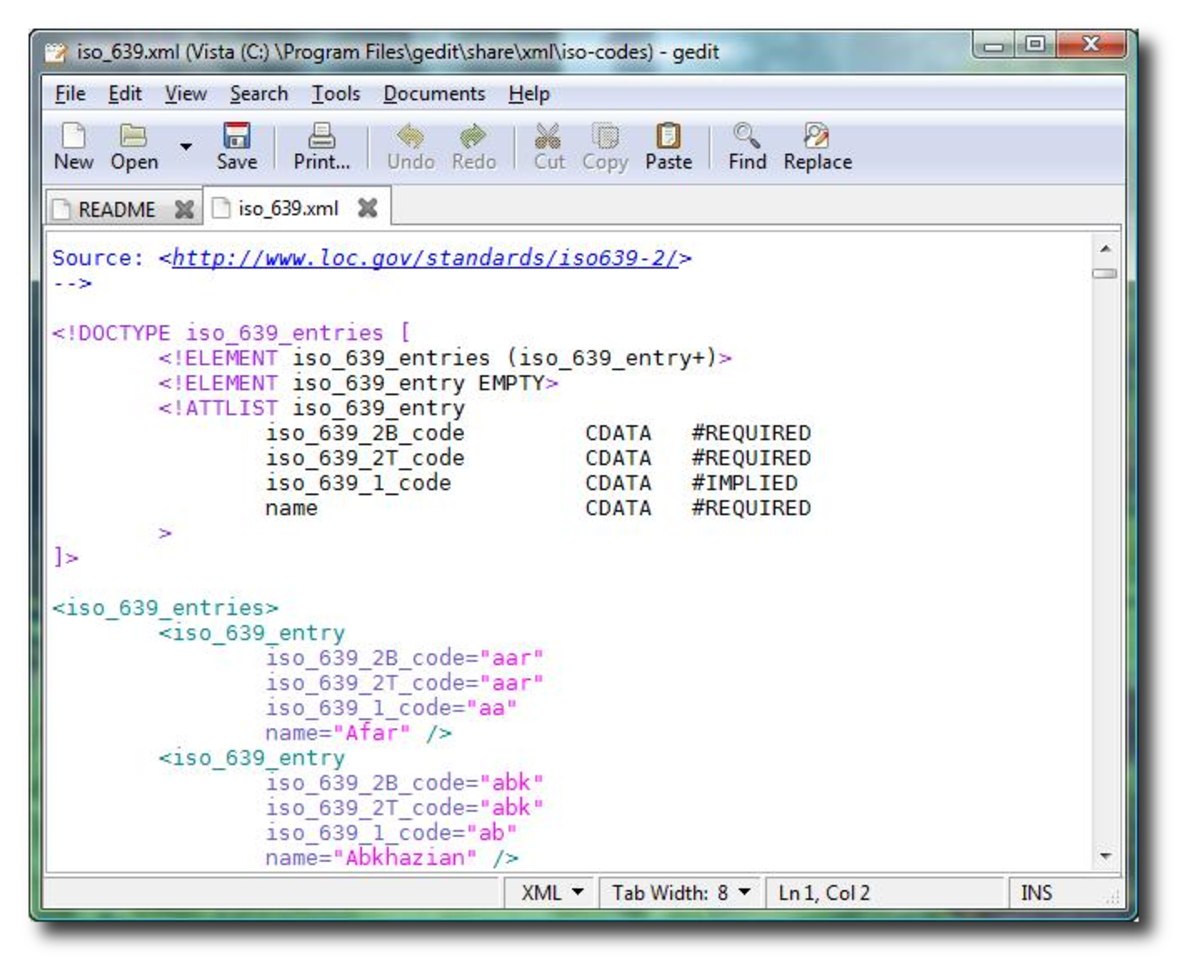
\includegraphics[scale=0.5]{gedit4.eps}<4>
	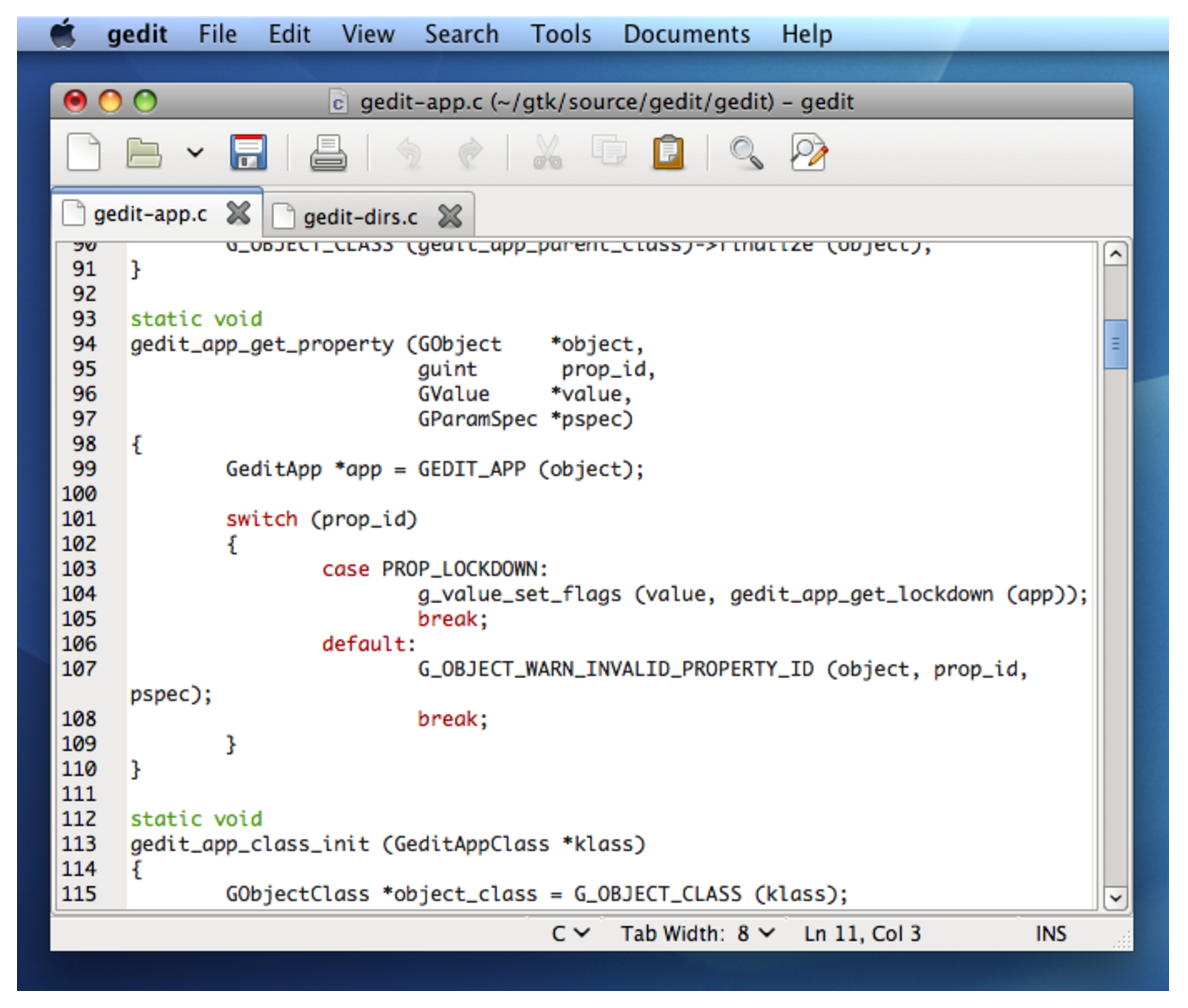
\includegraphics[scale=0.5]{gedit5.eps}<5>
\end{figure}
\end{frame}
\begin{frame}
\frametitle{El entorno Spyder2}
Spyder es un entorno de desarrollo integrado para el lenguaje \python\ con pruebas interactivas y funciones avanzadas de depuración, introspección y edición.
\\
\medskip
Spyder permite trabajar fácilmente con las mejores herramientas de la pila científica de \python\ en un entorno sencillo y potente.
\\
\medskip
\texttt{https://code.google.com/p/spyderlib/}
\end{frame}
\begin{frame}[fragile]
Estas son algunas de las características clave de Spyder:
\begin{enumerate}[<+->]
\item Cuadro de diálogo de administración de \texttt{PYTHONPATH} como de MATLAB (funciona con todas las consolas)
\item Editor de variables de entorno de usuario actual.
\item Enlaces directos a la documentación (\python, Matplotlib, NumPy, Spicy, etc.)
\item Enlace directo al lanzador de Python(x,y)
\item Enlaces directos a QtDesigner, QtLinguist y QtAssistant (documentación de Qt)
\end{enumerate}
\end{frame}
\begin{frame}
\begin{figure}
	\centering
	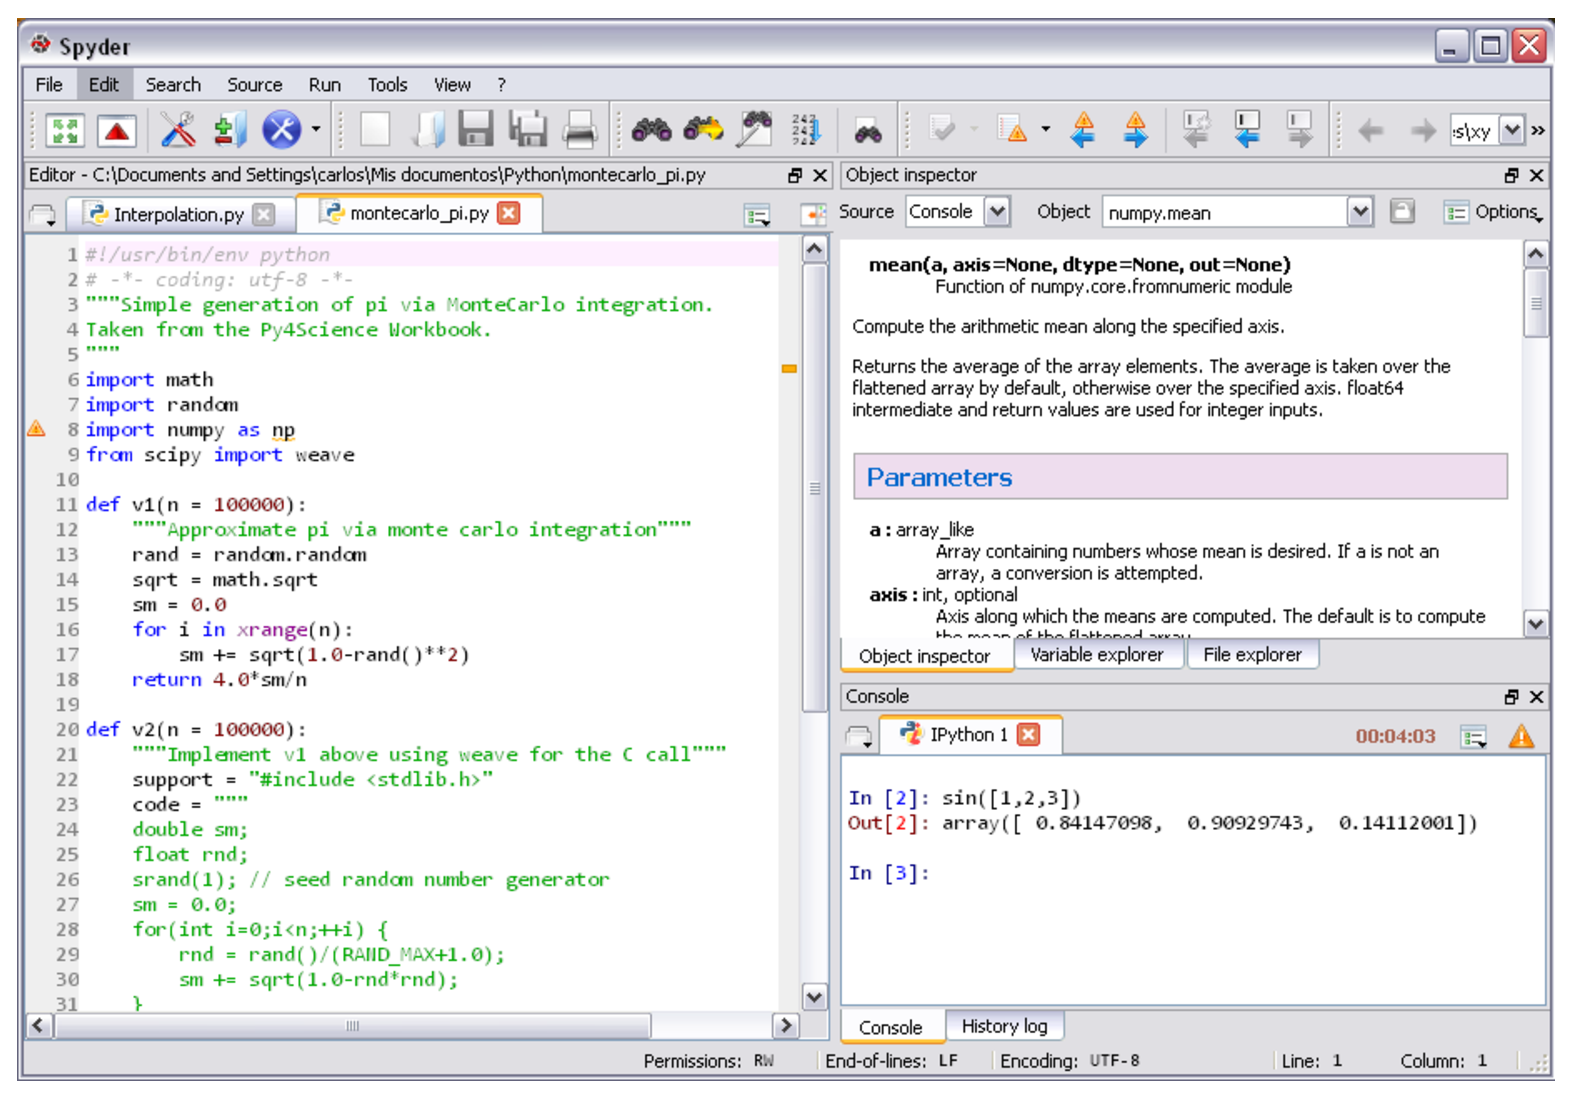
\includegraphics[scale=0.5]{spyder-windows.eps}<1>
	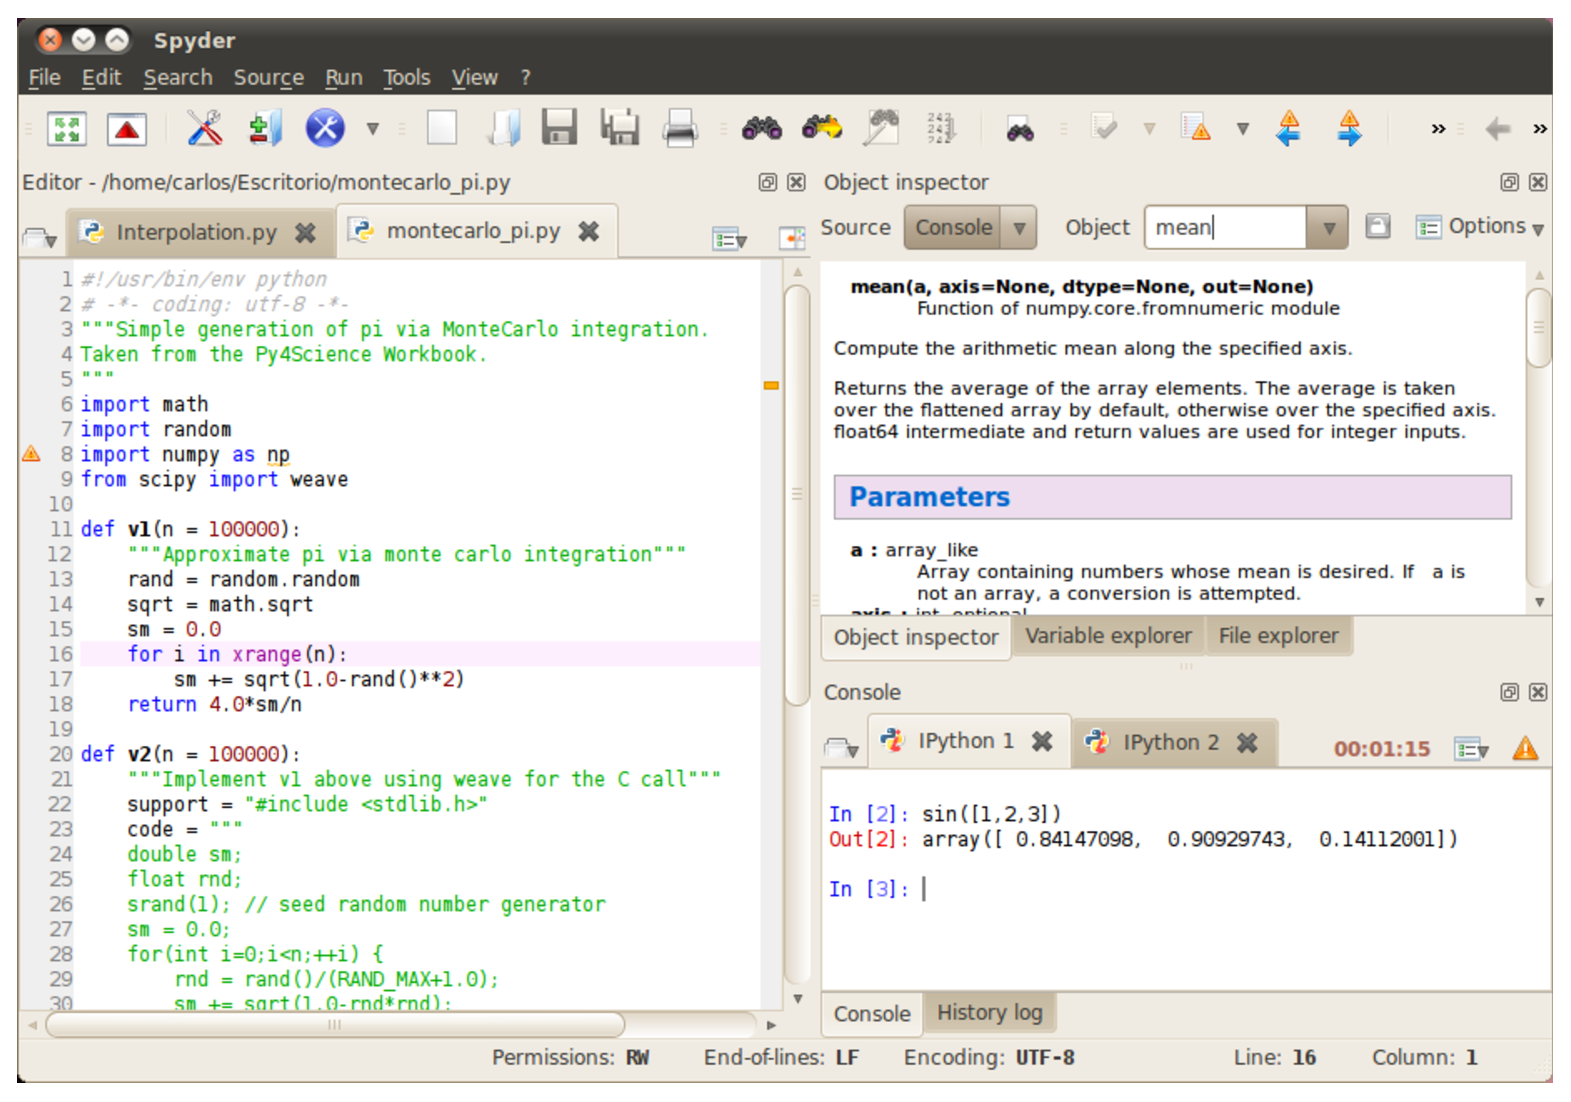
\includegraphics[scale=0.5]{spyder-linux.eps}<2> 
\end{figure}
\end{frame}
\begin{frame}
\frametitle{Otros IDEs para \python}
Pueden probar los IDE mencionados, pero también es importante señalar que hay otros entornos, cada uno con ciertas características que lo hacen particular. El punto es que si trabajan con uno, lo puedan explotar al máximo.
\\
\medskip
Una lista de otros IDEs para programar con \python, la pueden consultar en:
\\
\medskip
\texttt{https://wiki.python.org/moin/PythonEditors}
\end{frame}
\section{Funciones}
\begin{frame}
\frametitle{Funciones}
Con lo que hemos revisado sobre \python, tenemos elementos para iniciar la solución de problemas, una manera particular de agrupar un conjunto de instrucciones, es a través de funciones.
\\
\bigskip
Las funciones intrínsecas de cualquier lenguaje son pocas, pero podemos extenderlas con funciones definidas por el usuario.
\end{frame}
\begin{frame}[fragile]
\frametitle{Estructura de una función}
La estructura de una función en \python\ es la siguiente:
\begin{center}
\begin{exampleblock}{}
\verb| def nombre_funcion(parametro1, parametro2, ...):|
\verb|     conjunto de instrucciones|
\verb|     return valores_devueltos|
\end{exampleblock}
\end{center}
donde parametro1, parametro2 son los parámetros. Un parámetro puede ser cualquier objeto de \python, incluyendo una función.
\\
\medskip
Los parámetros pueden darse por defecto, por lo que en la función son opcionales. Si no se utiliza la instrucción \texttt{return}, la función devuelve un objeto \texttt{null}
\end{frame}
\begin{frame}[fragile]
\frametitle{Ejemplo}
\begin{lstlisting}
def cuadrados(a):
    for i in range(len(a)):
        a[i] = a[i]**2

a = [1, 2, 3, 4]
cuadrados(a)
print a
\end{lstlisting}
\end{frame}
\begin{frame}[fragile]
\frametitle{Paso de argumentos}
Para que una función sea en verdad útil (y reutilizable), es necesario que podamos pasarle entradas. Los nombres de las entradas (o argumentos) que requiere una función se declaran a continuación del nombre en \texttt{def} (siempre entre paréntesis)
\end{frame}
\begin{frame}[fragile]
\begin{verbatim}
def FuncionSuma (x, y):
    return x + y

print FuncionSuma (5, 3)
print FuncionSuma (7, 42.0)
print FuncionSuma (" hola ", " mundo ")
\end{verbatim}
\textbf{Nota:} 
\begin{itemize}
\item Nunca se mencionan los tipos de datos de x e y, ni el tipo de datos que devuelve FuncionSuma.
\item Los argumentos y el valor devuelto son, tal como las variables, simples etiquetas a zonas de memoria.
\end{itemize}  
\end{frame}
\begin{frame}[fragile]
\frametitle{Validar el tipo de dato}
A veces se va a requerir la validación del tipo de dato de manera explícita (aunque no es para nada pitónico!).
\\
\medskip
Un truco más o menos claro para emular lenguajes estáticos es usar la función \texttt{type} y la instrucción \texttt{assert}.
\end{frame}
\begin{frame}[fragile]
\begin{verbatim}
def SumaEnteros (x, y):
    assert type (x) == int
    assert type (y) == int
    return x+y
    
print SumaEnteros (5, 3) # -> 8
print SumaEnteros (7, 42.0) # -> AssertionError
\end{verbatim}
La instrucción \texttt{assert} actúaa como filtro si la expresión que le sigue es verdadera, pero falla con \texttt{AssertionError} si es falsa.
\\
\medskip
Es más común usar \texttt{try} y \texttt{except} para ''atrapar"" el error si los tipos no son los adecuados.
\end{frame}
\begin{frame}
\frametitle{Paso de argumentos con nombre}
Si la función que definimos tiene muchos argumentos, es fácil olvidar el orden en que fueron declarados.
\\
\medskip
Como un argumento no lleva asociado un tipo, \python no tiene manera de saber que los argumentos están cambiados.
\\
\medskip
Para evitar este tipo de errores, hay una manera de llamar a una función pasando los argumentos en cualquier orden arbitrario: se pasan usando el nombre usado en la declaración.
\end{frame}
\begin{frame}[fragile]
\begin{verbatim}
def Prueba (a, b, c):
# %r formatea automaticamente cualquier valor
    print "a= %r, b= %r, c= %r" % (a, b, c)

Prueba (1, 2, 3)
Prueba (b=3, a=2, c=1)

a=1, b=2, c=3
a=2, b=3, c=1
\end{verbatim}
\end{frame}
\begin{frame}[fragile]
\frametitle{Argumentos con valores por omisión}
Para hacer que algunos argumentos sean opcionales, se les da valores por omisión en el momento de declararlos:
\begin{verbatim}
from math import sqrt
# argumento v es requerido , c es opcional
# c toma el valor 3.0e8 por omision
def Gamma (v, c = 3.0e+8):
    return sqrt (1.0 -(v/c)**2)

print Gamma (0.1 , 1.0)
print Gamma (1.e+7) # usa c = 3.0e+8
\end{verbatim}
\end{frame}
\begin{frame}[fragile]
\frametitle{Regresando varios valores en una función}
Para hacer que una función devuelva más de un valor, en lenguajes como Fortran, C o C++, lo que se hace es definir argumentos de entrada y argumentos de salida.
\\
\medskip
Para devolver múltiples valores en \python, lo usual es devolver los valores ''empaquetados"" en una tupla:
\begin{verbatim}
from math import atan , sqrt

def ModuloArgumento (x, y):
    norm = sqrt (x**2 + y**2)
    arg = atan2 (y, x)
    return (norm,arg)
    
n, a = ModuloArgumento (3.0,4.0)
print " Modulo es:", n
print " Argumento es:", a
\end{verbatim}
\end{frame}
\begin{frame}[fragile]
\frametitle{Número variable de argumentos}
¿Cómo le hacemos para que una función acepte un número no prefijado de argumentos?
\\
\medskip
Es posible pasar una lista o tupla, pero \python\ ofrece una mejor solución:
\begin{verbatim}
def atan(*args ):
# args es una tupla de argumentos
    if len(args) == 1:
        return math.atan(args[0])
    else :
        return math.atan2(args[0],args[1])

print atan (0.2) # 0.19739
print atan (2.0,10.0) # 0.19739
print atan (-2.0,-10.0) # -2.94419
\end{verbatim}
\end{frame}
\begin{frame}
\frametitle{Cálculo de la serie de Fibonacci}
La sucesión fue descrita por Fibonacci como la solución a un problema de la cría de conejos: ''Cierto hombre tenía una pareja de conejos juntos en un lugar cerrado y uno desea saber cuántos son creados a partir de este par en un año cuando es su naturaleza parir otro par en un simple mes, y en el segundo mes los nacidos parir también''
\\
\bigskip
\pause
\textcolor{red}{cómo le hacemos?}
\end{frame}
\begin{frame}[fragile]
\frametitle{Propuesta de código}
\begin{lstlisting}
a, b = 0, 1
while b < 10:
    print b
    a, b = b, a+b
\end{lstlisting}
\pause
\begin{lstlisting}
a, b= 0, 1
while b < 1000:
    print b,
    a, b = b, a+b
\end{lstlisting}
\end{frame}
\section{Módulos}
\begin{frame}[fragile]
\frametitle{Módulos}
Es una buena práctica almacenar las funciones en módulos. Un módulo es un archivo en donde se dejan las funciones, el nombre del módulo es el nombre del archivo.
\\
\bigskip
Un módulo se carga al programa con la instrucción
\begin{center}
\verb|from nombre_modulo import *|
\end{center}
Python incluye un número grande de módulos que contienen funciones y métodos para varias tareas. La gran ventaja de los módulos es que están disponibles en internet y se pueden descargar, dependiendo de la tarea que se requiera atender.
\end{frame}
\begin{frame}[fragile]
\frametitle{Módulo \texttt{math}}
Muchas funciones matemáicas no se pueden llamar directo del intérprete, pero para ello existe el módulo \texttt{math}.
\\
\bigskip
Hay tres diferentes maneras en las que se puede llamar y utilizar las funciones de un módulo.
\begin{exampleblock}{}
\verb|from math import *|
\end{exampleblock}
De esta manera, se importan todas las funciones definidas en el módulo \texttt{math}, siendo quizá un gasto innecesario de recursos, pero también generar conflictos con definiciones cargadas de otros módulos.
\end{frame}
\begin{frame}[fragile]
\begin{exampleblock}{}
\verb|from math import func1, func2,...|
\end{exampleblock}
\pause
\begin{exampleblock}{}
\verb|>>> from math import log,sin| \\
\verb|>>> print log(sin(0.5))| \\
\verb|-0.735166686385|
\end{exampleblock}
\end{frame}
\begin{frame}[fragile]
El tercer método que es el más usado en programación, es tener disponible el módulo:
\begin{center}
\verb|import math|
\end{center}
Las funciones en el módulo se pueden usar con el nombre del módulo como prefijo:
\begin{exampleblock}{}
\verb|>>> import math| \\
\verb|>>> print math.log(math.sin(0.5))|
\verb|-0.735166686385|
\end{exampleblock}
\end{frame}
\begin{frame}[fragile]
\frametitle{Contenido del módulo \texttt{math}}
Podemos ver el contenido de un módulo con la instrucción:
\\
\verb|>>> import math| \\
\verb|>>> dir(math)|
\begin{verbatim}
['__doc__', '__name__', '__package__', 'acos',
'acosh',  'asin', 'asinh', 'atan', 'atan2',
'atanh', 'ceil', 'copysign', 'cos', 'cosh',
'degrees', 'e', 'erf', 'erfc', 'exp', 'expm1',
'fabs', 'factorial', 'floor', 'fmod', 'frexp',
'fsum', 'gamma', 'hypot', 'isinf', 'isnan',
'ldexp', 'lgamma', 'log', 'log10', 'log1p',
'modf', 'pi', 'pow', 'radians', 'sin', 'sinh',
'sqrt', 'tan', 'tanh', 'trunc']
\end{verbatim}
\end{frame}
\section{Graficación con \python}
\begin{frame}
\frametitle{Graficación con \python}
Una buena parte del trabajo que tendremos que hacer como físicos es utilizar un conjunto de datos que por si solos, no van a darnos información sobre un modelo o un fenómeno, por ello, será necesario usar gráficas.
\\
\medskip
\python incluye un módulo de graficación bastante versátil para generar gráficas y exportarlas a diferentes tipos de archivos.
\\
\medskip
La librería se llama \texttt{matplotlib}. Haremos algunos ejercicios para demostrar su potencia.
\end{frame}
\begin{frame}
\texttt{matplotlib.pyplot} es una colección de funciones de estilo de mando, de tal manera que matplotlib funciona a la manera de MATLAB. Cada instrucción \texttt{pyplot} aplica un cambio a una figura: por ejemplo, crear una figura, crear un área de trazado en una figura, trazar algunas líneas en un área de trazado, decorar con etiquetas, etc.
\end{frame}
\begin{frame}[fragile]
\frametitle{Ejecicio 1}
\begin{lstlisting}
import matplotlib.pyplot as plt
plt.plot([1,2,3,4])
plt.ylabel('algunos numeros')
plt.show()
\end{lstlisting}
\begin{figure}
	\centering
	\includegraphics[scale=0.35]{plotEjercicio1.eps}<2> 
\end{figure}
\end{frame}
\begin{frame}
Te estarás preguntando por qué tenemos en el eje $x$ el rango $0-3$ y en el eje $y$ el rango  $1-4$.
\\
\medskip
Si proporcionamos una única lista o matriz en el comando \texttt{plot}, \texttt{matplotlib} asume que es una secuencia de valores de $y$, por lo que genera automáticamente los valores de $x$ para nosotros. Como los índices en \python comienzan en $0$, el vector $x$ por defecto tiene la misma longitud que $y$, pero inicia con 0. De ahí que los datos $x$ son $[0,1,2,3]$.
\end{frame}
\begin{frame}[fragile]
\frametitle{Ejecicio 2}
\begin{lstlisting}
import matplotlib.pyplot as plt
plt.plot([1,2,3,4], [1,4,9,16], 'ro')
plt.axis([0, 6, 0, 20])
plt.show()
\end{lstlisting}
\begin{figure}
	\centering
	\includegraphics[scale=0.35]{plotEjercicio2.eps}<2> 
\end{figure}
\end{frame}
\begin{frame}[fragile]
Por cada par $x$, $y$ de argumentos, existe un tercer argumento opcional, que es la cadena de formato que indica el color y tipo de línea.
\\
\medskip
Las letras y los símbolos de la cadena de formato son como en MATLAB, y concatenar una cadena de color con una cadena estilo de línea.
\\
\medskip
La cadena de formato por defecto es \verb|'b-'|, que es una línea de color azul.
\end{frame}
\begin{frame}[fragile]
\frametitle{Tipos de líneas}
\begin{tabular}{l | l}
carácter & descripción \\ \hline
\verb|'-'|	& línea sólida \\ \hline
\verb|'--'| & línea cortada \\ \hline
\verb|'-.'| & línea-punto \\ \hline
\verb|':'|	& línea de puntos \\ \hline
\verb|'.'|	& marca de punto \\ \hline
\verb|','|	& marca de pixel \\ \hline
\verb|'o'|	& marca de círculo \\ \hline
\verb|'v'|	& marca de triándulo hacia abajo \\ \hline
\verb|'^'|	& marca de triángulo hacia arriba
\end{tabular}
\end{frame}
\begin{frame}[fragile]
\frametitle{Lista de colores}
\begin{tabular}{l | l}
carácter & color \\ \hline
\verb|'b'| & azul \\ \hline
\verb|'g'| & verde \\ \hline
\verb|'r'| & rojo \\ \hline
\verb|'c'| & cyan \\ \hline
\verb|'m'| & magenta \\ \hline
\verb|'y'| & amarillo \\ \hline
\verb|'k'| & negro \\ \hline
\verb|'w'| & blanco
\end{tabular}
\end{frame}
\begin{frame}
\texttt{matplotlib} se limita a trabajar con listas, por lo que sería bastante acotado para el procesamiento y análisis numérico.
\\
\medskip
Por lo general, se utilizan los arreglos del módulo \texttt{numpy}. De hecho, todas las secuencias se convierten en matrices de \texttt{numpy} internamente.
\\
\medskip
El siguiente ejemplo ilustra un trazado de líneas con varios estilos diferentes en una sola instucción utilizando arreglos.
\end{frame}
\begin{frame}[fragile]
\frametitle{Ejecicio 3}
\begin{lstlisting}
import numpy as np
import matplotlib.pyplot as plt

t = np.arange(0., 5., 0.2)
plt.plot(t, t, 'r--', t, t**2, 'bs', t, t**3, 'g^')
plt.show()
\end{lstlisting}
\end{frame}
\begin{frame}[fragile]
\begin{figure}
	\centering
	\includegraphics[scale=0.5]{plotEjercicio3.eps}
\end{figure}
\end{frame}
\begin{frame}[fragile]
\frametitle{Ejercicio 4}
Trabajando con múltiples gráficas
\begin{lstlisting}
import numpy as np
import matplotlib.pyplot as plt

def f(t):
    return np.exp(-t) * np.cos(2*np.pi*t)

t1 = np.arange(0.0, 5.0, 0.1)
t2 = np.arange(0.0, 5.0, 0.02)

plt.figure(1)
plt.subplot(211)
plt.plot(t1, f(t1), 'bo', t2, f(t2), 'k')

plt.subplot(212)
plt.plot(t2, np.cos(2*np.pi*t2), 'r--')
\end{lstlisting}
\end{frame}
\begin{frame}[fragile]
\begin{figure}
	\centering
	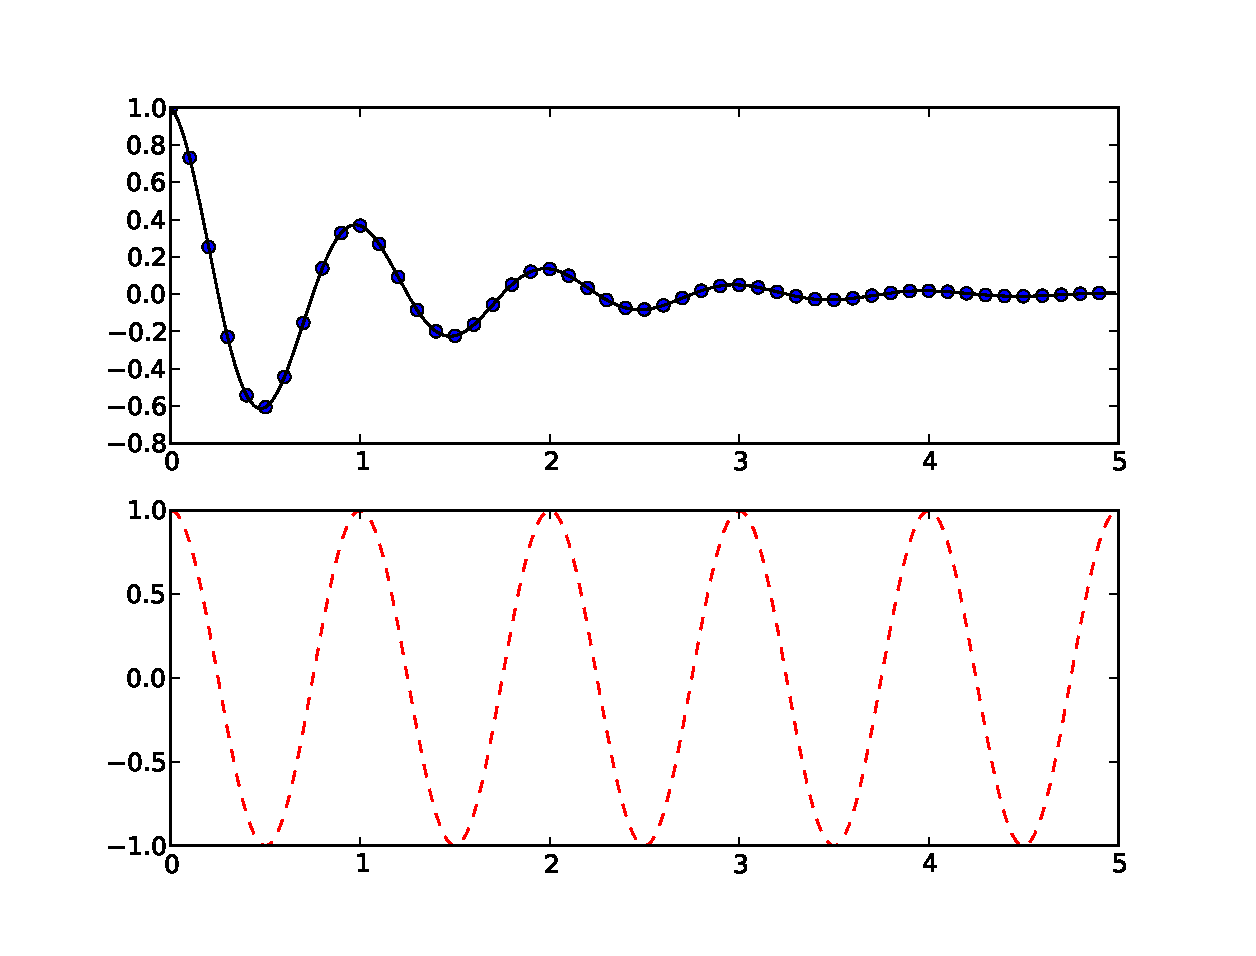
\includegraphics[scale=0.5]{plotEjercicio4.eps}
\end{figure}
\end{frame}
\begin{frame}
El comando \texttt{figure()} aquí es opcional, ya \texttt{figure(1)} se crea de forma predeterminada, así mismo \texttt{subplot(111)} se crea de forma predeterminada si no se especifica manualmente un eje.
\\
\medskip
El comando \texttt{subplot()} especifica \texttt{numrows, numcols, fignum} donde \texttt{fignum} varía en rango de 1 a \texttt{numrows * numcols}. Las comas en el comando \texttt{subplot()} son opcionales si \texttt{numrows * numcols} $<10$. Por tanto \texttt{subplot(211)} es idéntica a la \texttt{subplot(2,1,1)}.
\end{frame}
\begin{frame}[fragile]
\frametitle{Ejercicio 5}
\begin{lstlisting}
import matplotlib.pyplot as plt

plt.figure(1)                
plt.subplot(211)         
plt.plot([1,2,3])
plt.subplot(212)         
plt.plot([4,5,6])


plt.figure(2)                
plt.plot([4,5,6])           

plt.figure(1)                
plt.subplot(211)         
plt.title('Tan facil como 1,2,3')
plt.show()
\end{lstlisting}
\end{frame}
\begin{frame}[fragile]
\begin{figure}
	\centering
	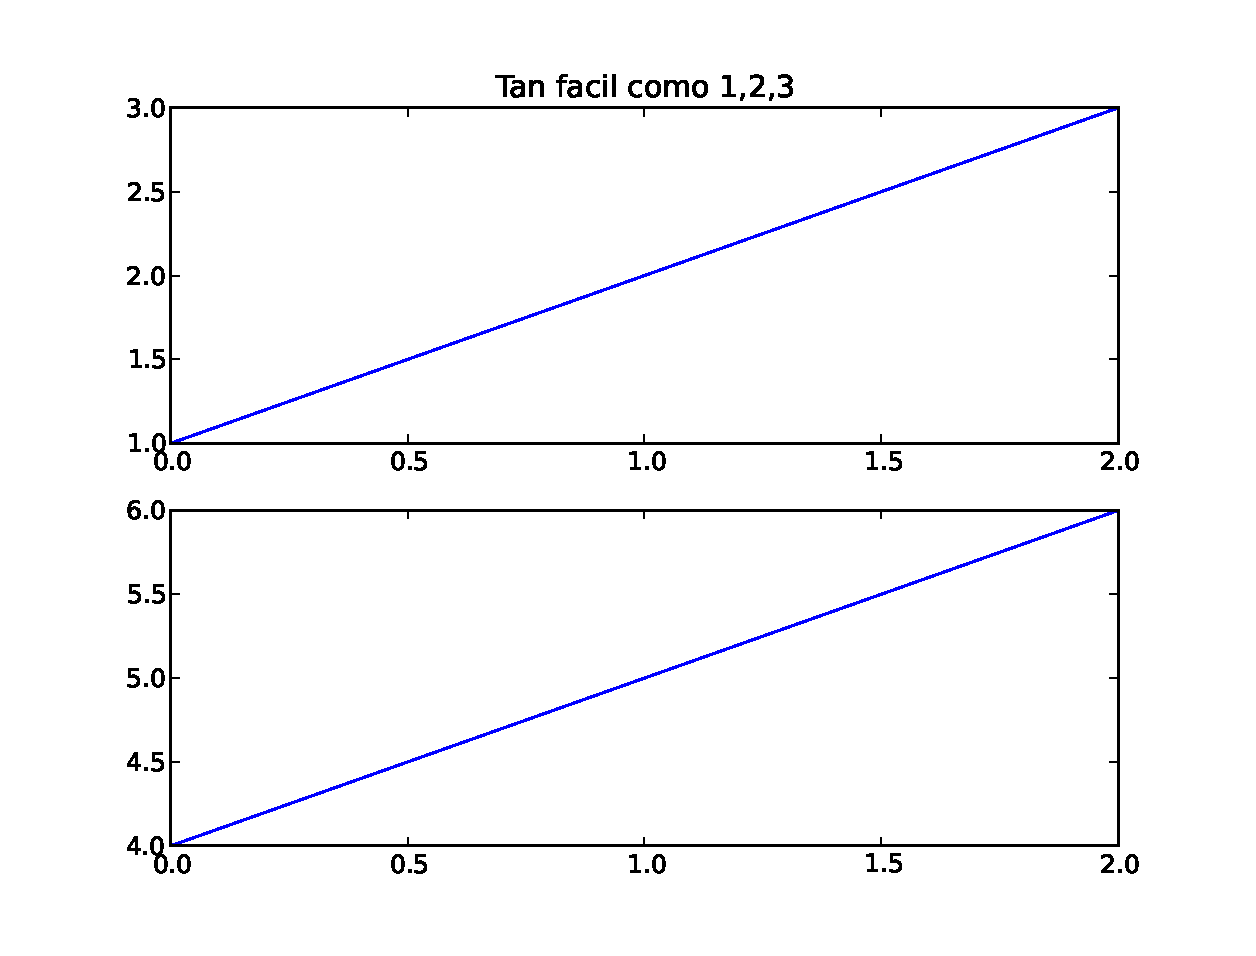
\includegraphics[scale=0.5]{plotEjercicio5_1.eps}<1>
	\includegraphics[scale=0.5]{plotEjercicio5_2.eps}<2>
\end{figure}
\end{frame}
\section{Primeros problemas de la física}
\begin{frame}
\frametitle{Primeros problemas de la física}
De manera paralela a los conceptos importantes del curso, es necesario iniciar el trabajo de plantear algoritmos de solución a problemas de la física.
\\
\medskip
La mejor manera de aprender, es sentarse a programar. Debe de tenerse la calma para ello, la idea es ir perfeccionando las propuestas de solución, es importante señalar que la inspiración divina, no se da siempre.
\end{frame}
\begin{frame}[fragile]
\frametitle{Proceso de programación}
El proceso de programación consta de las actividades necesarias para escribir programas que funcionen adecuadamente como solución a un problema particular. \footnote{Amparo López Gaona, \textit{Introducción al desarrollo de programas con Java}, 3a. Ed., La Prensa de Ciencias, México D.F. 2013.}
\begin{enumerate}[<+->]
\item Definición del problema.
\item Diseño de la solución.
\item Codificación.
\item Depuración.
\item Mantenimiento.
\end{enumerate}
\end{frame}
\begin{frame}
\frametitle{Definición del problema}
Aquí se especifica qué es lo que debe de hacer el programa.
\\
\bigskip
Este primer paso puede parecer trivial aunque no lo es. La comprensión exacta de lo que se necesita hacer es requisito indispensable para crear una solución funcional.
\\
\medskip
En ocasiones, se ignora esta fase y se comienza a escribir un programa sin tener en claro el problema a resolver.
\end{frame}
\begin{frame}
\frametitle{Diseño de la solución}
En esta fase se indica una forma de satisfacer, mediante un programa, los requerimientos establecidos en la etapa anterior.
\\
\bigskip
El diseño de un programa es un proceso al que muchas veces no se le da la importancia y de ahí que en las etapas posteriores se tengan muchos problemas.
\\
\medskip
En el diseño es necesario identificar los principales componentes de la solución y la relación entre ellos.
\end{frame}
\begin{frame}
\frametitle{Codificación}
Una vez que se tiene el diseño de la solución, se procede a traducirlo a un lenguaje de programación.
\\
\bigskip
Esta tarea se conoce como codificación o implementación. En muchas ocasiones, uno se centra únicamente en esta etapa aunque, como se puede ver, el proceso de programar es mucho más complejo y creativo.
\end{frame}
\begin{frame}[fragile]
Es recomendable acostumbrarse desde el inicio a escribir programas que sean fácilmente entendibles por otras personas; podemos apoyarnos con lo siguiente:
\begin{enumerate}[<+->]
\item Los programas deben de tener una estructura clara.
\item El código debe estar organizado y presentado de manera que sea fácil su lectura.
\item El código debe de estar documentado.
\end{enumerate}
\end{frame}
\begin{frame}
\frametitle{Depuración}
El siguiente paso en el desarrollo de un programa es la depuración que consiste en verificar que el algoritmo y el programa sean adecuados. No importa que tan bonito esté el programa, si no produce los resultados deseados, simplemente no sirve.
\\
\bigskip
Depurar implica descubrir, localizar y corregir todos los errores que causen que un programa produzca resultados incorrectos o que no produzca ningún resultado.
\end{frame}
\begin{frame}
\frametitle{Mantenimiento}
En los programas y trabajos escolares, la tarea termina en el paso anterior, pero en la vida real no es así. La etapa de mantenimiento consiste en supervisar la operación de un programa, corregir cualquier error encontrado durante su uso continuo o efectuar modificaciones al mismo, con el propósito de que realice más tareas o de manera diferente a las que tenían contempladas originalmente.
\end{frame}
\subsection{Ejercicios de Mecánica}
\begin{frame}
\frametitle{Un primer problema de Mecánica}
Supongamos que tenemos una partícula de masa $m$ que está confinada a moverse a lo largo del eje $x$, bajo una fuerza $f(x)$. Sabemos de la ley de Newton que
\begin{equation}\label{Eqfuerza}
f = ma = m \dfrac{dv}{dt}
\end{equation}
donde $a$ es la aceleración y $v$ la velocidad de la partícula respectivamente, $t$ es el tiempo.
\\
\medskip
Si dividimos el tiempo en pequeños intervalos iguales $\tau = t_{i+1} - t_{i}$, sabemos que la velocidad en el tiempo $t_{i}$, está dada de manera aproximada por el promedio de la velocidad en el intervalo de tiempo $[t_{i}, t_{i+1}]$
\end{frame}
\begin{frame}
Por lo que
\begin{equation}\label{Eqvelocidad}
v_{i} \simeq \dfrac{x_{i+1}-x_{i}}{t_{i+1}-t_{i}} = \dfrac{x_{i+1}-x_{i}}{\tau}
\end{equation}
La aceleración de la partícula es aproximadamente el promedio de la aceleración en el mismo intervalo
\begin{equation}\label{Eqaceleracion}
a_{i} \simeq \dfrac{v_{i+1}-v_{i}}{t_{i+1}-t_{i}} = \dfrac{v_{i+1}-v_{i}}{\tau}
\end{equation}
donde $\tau$ es muy pequeño.
\end{frame}
\begin{frame}
El algoritmo más sencillo para determinar la posición y velocidad de la partícula en el tiempo $t_{1i+1}$, a partir de las cantidades correspondientes al tiempo $t_{i}$, se obtiene luego de combinar las ecuaciones (\ref{Eqfuerza}), (\ref{Eqvelocidad}) y (\ref{Eqaceleracion}), por lo que
\begin{eqnarray}
x_{i+1} &=& x_{i} + \tau v_{i} \label{Eqposicion} \\
v_{i+1} &=& v_{i} + \dfrac{\tau}{m} f_{i} \label{Eqvelocidadr}
\end{eqnarray}
donde $f_{i} = f(x_{i})$
\end{frame}
\begin{frame}
Si se proporciona la posición inicial y la velocidad de la partícula y se buscan las cantidades correspondientes en algún momento posterior (problema de valor inicial), podemos obtenerlas de forma recursiva a partir del algoritmo dado en las ecuaciones (\ref{Eqposicion}) y (\ref{Eqvelocidadr}).
\end{frame}
\subsection{Ejercicio 1: Oscilador mecánico}
\begin{frame}
\frametitle{Ejercicio 1: Oscilador mecánico}
Por simplicidad, consideremos que la fuerza es $f(x) = -kx$, donde $k$ es la constante del resorte. Usemos $m=k=1$. Queremos describir la posición y velocidad de la partícula en un intervalo de tiempo de 100 segundos. Las condiciones iniciales son las siguientes: $x(t=0) = 0$ y $v(t=0) = 1$.
\end{frame}
\begin{frame}[<+->]
\frametitle{Resolviendo el problema con Python}
¿Qué es lo que tenemos?
\begin{itemize}
\item El intervalo de tiempo de $[0,100]$ segundos.
\item La posición y velocidad inicial.
\item Las expresiones para calcular los $x_{i+1}$ y $v_{i+1}$
\end{itemize}
\visible<4->{¿Qué nos falta?}
\end{frame}
\begin{frame}[fragile]
\frametitle{Lo que nos falta}
\begin{itemize}[<+->]
\item Calcular para cada segundo en $[0,100]$ la posición y velocidad.
\item Guardar esos valores en un algún lado.
\item Graficar los resultados.
\end{itemize}
\end{frame}
\begin{frame}[fragile]
\frametitle{Uso de los módulos para nuestro programa}
Para graficar con el módulo \texttt{matplotlib} incluido en Python, necesitamos llamar a la librería \texttt{pyplot}, para acortar la escritura, usamos un \emph{alias}, en este caso \texttt{plt}.
\begin{lstlisting}
import matplotlib.pyplot as plt
from math import pi
\end{lstlisting}
\end{frame}
\begin{frame}[fragile]
\frametitle{Usando la información que nos proporciona el problema}
\begin{lstlisting}
n = 100

x = []
v = []

dt = 2* pi/n

x.append(0)
v.append(1)
\end{lstlisting}
\end{frame}
\begin{frame}[fragile]
\frametitle{Ciclo de iteración para los nuevos valores}
Como la fuerza en este caso es del tipo $f(x) = -kx$, tenemos un cambio de signo en el segundo sumando de $vi$.
\begin{lstlisting}
for i in range(n-1):
    xi = x[i] + v[i]*dt
    vi = v[i] - x[i]*dt
    
    x.append(xi)
    v.append(vi)
\end{lstlisting}
\end{frame}
\begin{frame}[fragile]
\frametitle{Generación de una gráfica}
La instrucción \texttt{plot}, nos permite crear en una nueva ventana, la gráfica, en este caso, requiere de una variable para poder desplegar los valores contenidos en la lista; el parámetro ''ro-'' lo usamos para decirle a matplotlib que nos devuelva una línea roja, con el símbolo ''o'', que estará ''unido'' entre sí por cada valor de la lista, además le agregamos una etiqueta para identificar nuestra gráfica. Hacemos lo mismo para la otra gráfica que nos representa la velocidad de la masa, ahora con color azul y el símbolo ''+''.
\begin{lstlisting}
plt.plot(x, "ro-", label="Posicion")
plt.plot(v, "b+-", label="Velocidad")
plt.legend(loc="upper right")
plt.xlabel("tiempo")
plt.show()
\end{lstlisting}
\end{frame}
\begin{frame}
\frametitle{Resultado del problema}
\begin{figure}
	\centering
	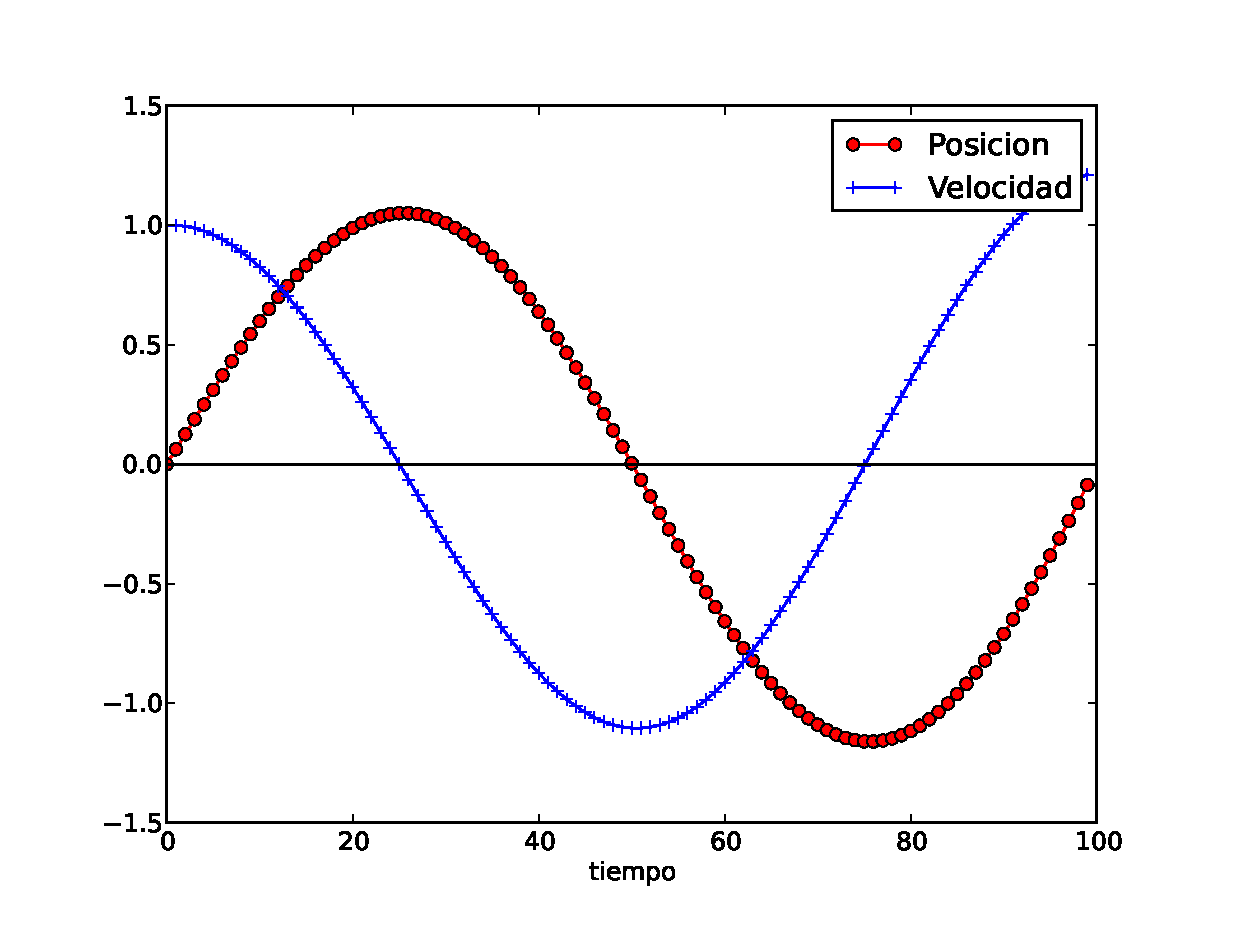
\includegraphics[scale=0.5]{Imagenes/EjerMecanica01.eps} 
\end{figure}
\end{frame}
\subsection{Ejercicio 2: Efecto de la resistencia del aire}
\begin{frame}
\frametitle{Ejecicio 2: Efecto de la resistencia del aire}
La bicicleta es una forma muy eficiente de transporte, este es un hecho bien conocido por cualquier persona que monta una. Nuestro objetivo en este ejercicio es comprender los factores que determinan la velocidad máxima de una bicicleta y estimar la velocidad de un caso real.
\\
\bigskip
Comenzaremos haciendo caso omiso de la fricción; tendremos que añadirlo al final, por supuesto, pero debemos primero entender cómo lidiar con el caso más simple y sin fricción.
\end{frame}
\begin{frame}
La ecuación de movimiento corresponde a la segunda ley de Newton, que escribimos de la forma
\begin{equation}\label{EqNewton2}
\dfrac{dv}{dt} = \dfrac{F}{m}
\end{equation}
donde $v$ es la velocidad, $m$ es la masa de la combinación de la bicicleta-conductor, $t$ es el tiempo, y $F$ es la fuerza en la bicicleta que viene del esfuerzo del conductor (en este caso vamos a suponer que la bicicleta se mueve sobre un terreno plano)
\end{frame}
\begin{frame}
Tratar correctamente a $F$ se complica por la mecánica de la bicicleta, ya que la fuerza ejercida por el ciclista se transmite a las ruedas por medio del plato, engranajes, cadena, etc. Esto hace que sea muy difícil derivar una expresión exacta para $F$.
\\
\medskip
Sin embargo, hay otra manera de abordar este problema que evita la necesidad de conocer la fuerza. Este enfoque alternativo implica la formulación del problema en términos de la potencia generada por el ciclista.
\\
\medskip
Estudios fisiológicos de ciclistas de carreras han demostrado que estos atletas son capaces de producir una potencia de salida de aproximadamente 400 watts durante largos períodos de tiempo ($\sim 1$ h)
\end{frame}
\begin{frame}
Usando las ideas de trabajo-energía podemos reescribir (\ref{EqNewton2}) como
\begin{equation}\label{EqPotencia}
\dfrac{dE}{dt} = P
\end{equation}
donde $E$ es la energía total, $P$ es la potencia de salida del ciclista. Para un trayecto plano la energía es totalmente cinética, es decir, $E = \frac{1}{2} m v^{2}$, y $\frac{dE}{dt} = mv (\frac{dv}{dt})$, usando esto en (\ref{EqPotencia}), resulta
\begin{equation}\label{EqPotenciavel}
\dfrac{dv}{dt} = \dfrac{P}{mv}
\end{equation}
\end{frame}
\begin{frame}
Si $P$ es una constante, la ecuación (\ref{EqPotenciavel}), se puede resolver de manera analítica, rearreglando términos:
\begin{equation}\label{EqIntegral}
\int_{v_{0}}^{v} v' dv' = \int_{0}^{t} \dfrac{P}{m} dt'
\end{equation}
donde $v_{0}$ es la velocidad de la bicicleta en $t=0$. Integrando ambos lados de la ecuación y resolviendo para $v$, tenemos
\begin{equation}\label{Eqvres}
v = \sqrt{v_{0}^{2} + 2 P \dfrac{t}{m}}
\end{equation}
\end{frame}
\begin{frame}[fragile]
\frametitle{Considera lo siguiente}
\begin{verbatim}
t = []
v = []

dt = 1

potencia = 400

masa = 70

tmax = 200

nmax = tmax/dt


t.append(0)
v.append(4)
\end{verbatim}
\end{frame}
\begin{frame}
\frametitle{Resultado de la velocidad sin fricción}
\begin{figure}
	\centering
	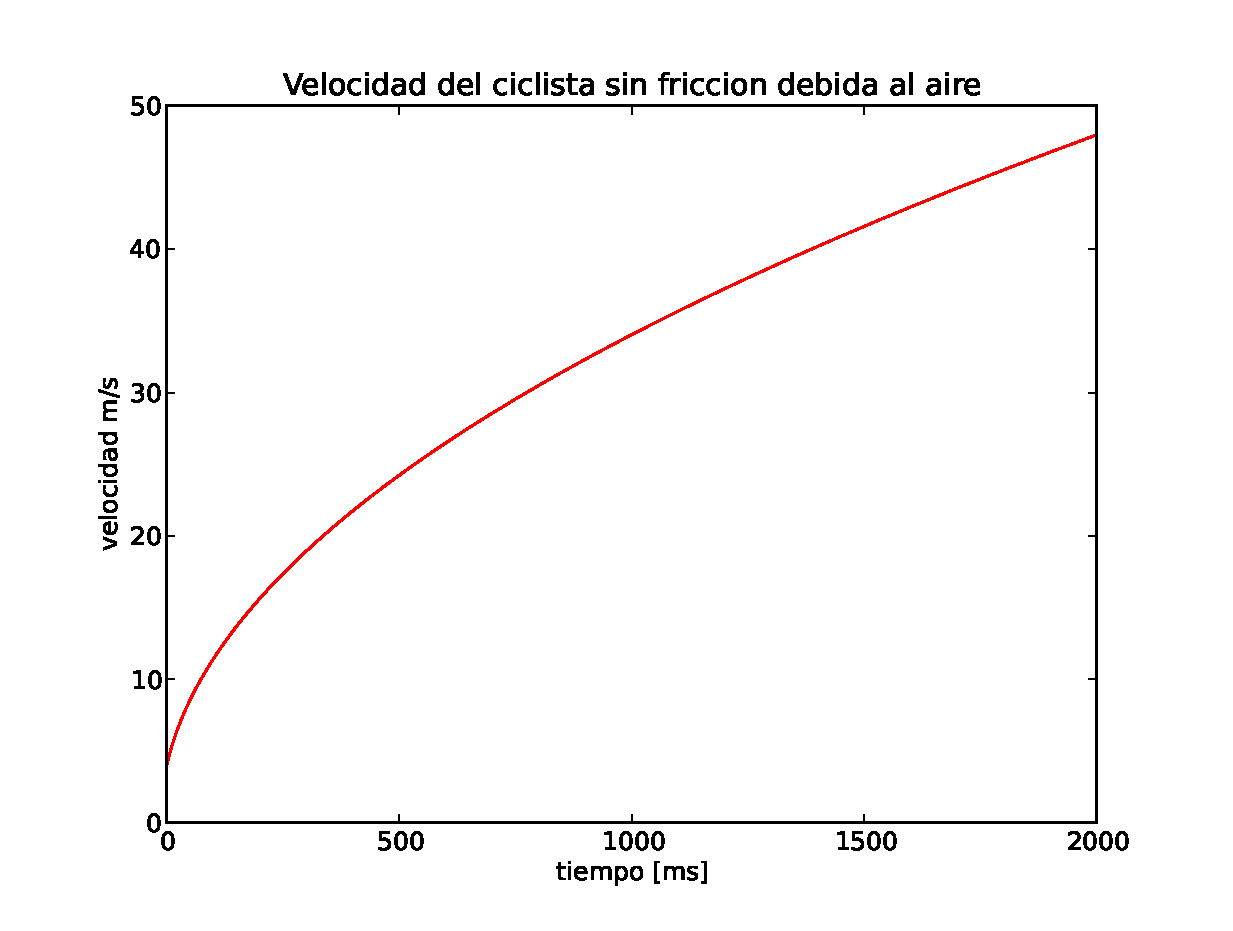
\includegraphics[scale=0.5]{EjerBicicleta01.eps}
\end{figure}
\end{frame}
\begin{frame}
Si bien esta es la solución correcta de la ecuación de movimiento (\ref{EqPotenciavel}), nuestro trabajo no concluye aquí, ya que predice que la velocidad se incrementará sin límite para tiempos muy largos.
\\
\medskip
Vamos a corregir este resultado, cuando se generaliza el modelo se debe de incluir el efecto de la resistencia del aire. El nuevo término que vamos a añadir a la ecuación de movimiento nos obliga a desarrollar una solución numérica, así que con eso en mente se considera un tratamiento numérico de (\ref{EqPotenciavel})
\end{frame}
\begin{frame}
Comenzamos con la forma de diferencias finitas para la derivada de la velocidad
\begin{equation}\label{Eqderivada}
\dfrac{dv}{dt} \simeq \dfrac{v_{i+1}-v_{i}}{\Delta t}
\end{equation}
donde asumimos que $\Delta t$ es paso discreto pequeño, y $v_{i}$ es la velocidad al tiempo $t_{i} \equiv i \Delta t$, por lo que de la ecuación (\ref{EqPotenciavel})
\begin{equation}\label{Eqveli+1}
v_{i+1} = v_{i} + \dfrac{P}{m v_{i}} \Delta t
\end{equation}
\end{frame}
\begin{frame}
Dada la velocidad en un tiempo $i$ (es decir, $v_{i}$), podemos usar (\ref{Eqveli+1}) para calcular un valor \textit{aproximado} de la velocidad en el siguiente paso $v_{i+1}$.
\\
\medskip
Si conocemos la velocidad inicial $v_{0}$, podemos obtener $v_{1}$, $v_{2}$, y así sucecivamente.
\end{frame}
\begin{frame}
\frametitle{Considerando la fricción del aire}
La fuerza debida a la fricción puede aproximarse de manera inicial como
\begin{equation}\label{EqFfriccion}
F_{a} \simeq - B_{1} v - B_{2} v^{2}
\end{equation}
Para velocidades muy bajas, el primer término es el que domina, y el coeficiente $B_{1}$ se puede calcular para objetos con formas sencillas.
\\
\medskip
Para una velocidad razonable $v^{2}$ el término domina sobre los demás, pero $B_{2}$ no puede calcularse exactamente en objetos sencillos como una pelota de beisbol, menos para una bicicleta.
\end{frame}
\begin{frame}
Podemos aproximar el valor de $B_{2}$ como sigue:
\\
\medskip
Si un objeto se mueve a través de la atmósfera y debe empujar fuera del camino el aire delante de él. La masa de aire movido en el tiempo $dt$ es $m_{aire} \sim \rho Avdt$, donde $\rho$ es la densidad del aire y $A$ el área frontal del objeto. A este aire se le da una velocidad de orden $v$, y por lo tanto, su energía cinética es $E_{aire} \sim m_{aire} v^{2} /2$
\\
\medskip
Este es también el trabajo realizado por la fuerza de arrastre (la fuerza sobre el objeto debido a la resistencia del aire) en el tiempo $dt$, por lo $F_{a}vdt = E_{aire}$. Poniendo todo esto junto nos encontramos
\[ F_{a} \simeq - C \rho A v^{2} \]
\end{frame}
\begin{frame}
Incluyendo este término en la expresión para la velocidad
\begin{equation}\label{Eqvelifriccion}
v_{i+1} = v_{i} + \dfrac{P}{m v_{i}} \Delta t - \dfrac{C \rho A v_{i}^{2}}{m} \Delta t
\end{equation}
Ahora te toca implementar el código, considerando $C = 0.5$ y $A=0.33$
\end{frame}
\begin{frame}
\frametitle{Comparando velocidades}
\begin{figure}
	\centering
	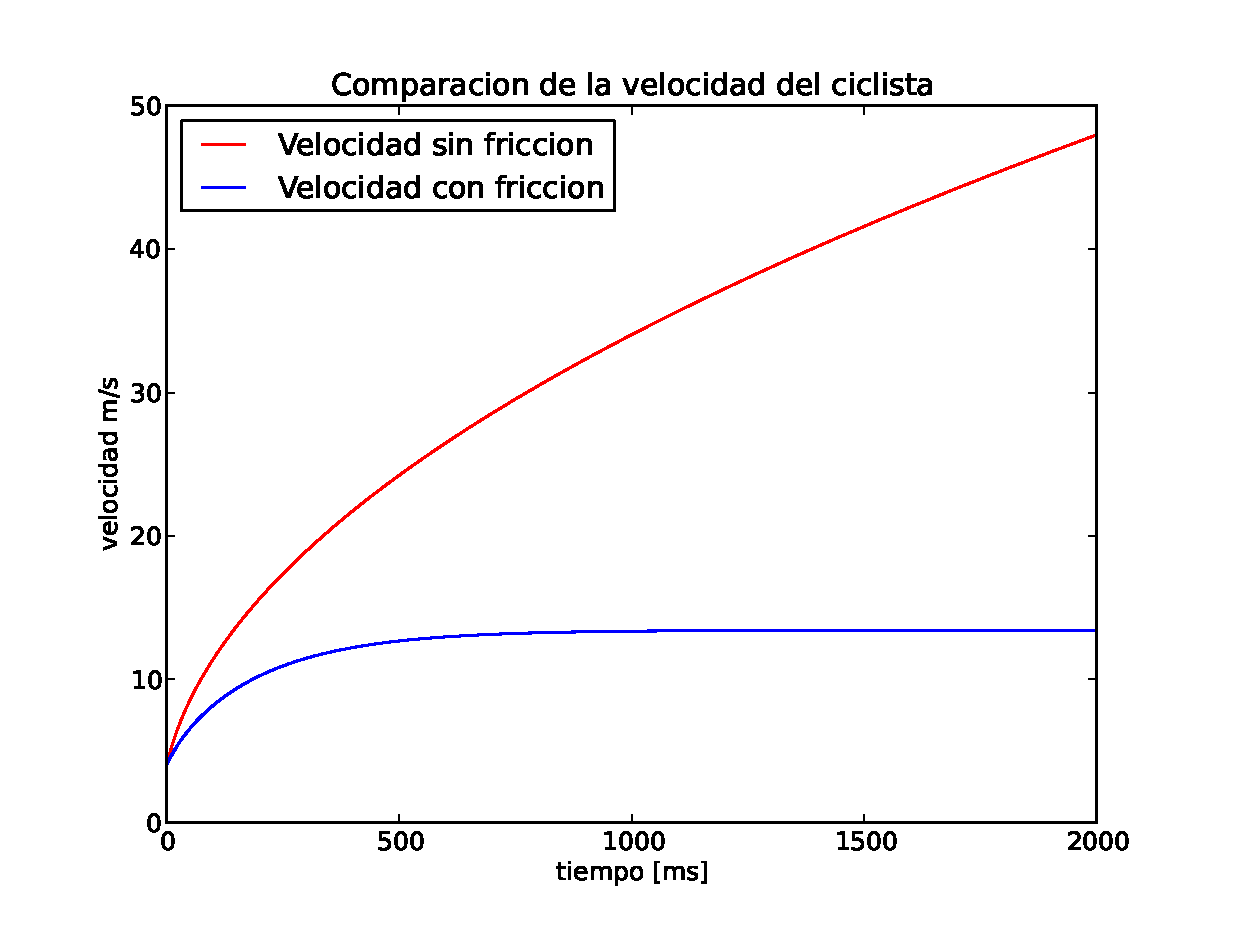
\includegraphics[scale=0.5]{EjerBicicleta02.eps}
\end{figure}
\end{frame}
\end{document}